% ==========================================
% Step 4/4 - Final refinement (refinement step 3)
% Output: step4-02-25-2026-wednesday-week2-Analysis_II-_mehrere_Variablen-offset-final-copy1.tex
% Input: step3-02-25-2026-wednesday-week2-Analysis_II-_mehrere_Variablen-offset-speech_refined.tex
% Model: gemini-3.8-flash
% Temperature: 0.35
% TopP: 0.9
% TopK: 10
% MaxOutputTokens: 65535
% ThinkingBudget: 4096
% ThinkingLevel: MEDIUM
% Processed on: 2026-10-12 21:59:32
% ------------------------------------------
% Token Usage (1 Request(s)):
%   - Total Prompt Tokens : 71'632 (gesamter Prompt, inkl. Cache)
%   - Cached Context      : 0 (aus Google Context-Cache, rabattiert)
%   - Fresh Input Tokens  : 71'632 (neu verrechneter Input)
%   - Output Tokens       : 37'527 (generiertes LaTeX, ohne Thinking)
%   - Thinking Tokens     : 9'020 (Denk-Tokens, als Output verrechnet)
% ==========================================
% ==========================================
% Step 3/4 - Speech refinement (refinement step 2)
% Output: step3-02-25-2026-wednesday-week2-Analysis_II-_mehrere_Variablen-offset-speech_refined.tex
% Input: step2-02-25-2026-wednesday-week2-Analysis_II-_mehrere_Variablen-offset-merged.tex
% Model: gemini-3.8-flash
% Temperature: 0.35
% TopP: 0.9
% TopK: 10
% MaxOutputTokens: 65535
% ThinkingBudget: 4096
% ThinkingLevel: MEDIUM
% Processed on: 2026-10-12 21:34:23
% ------------------------------------------
% Token Usage (1 Request(s)):
%   - Total Prompt Tokens : 232'316 (gesamter Prompt, inkl. Cache)
%   - Cached Context      : 0 (aus Google Context-Cache, rabattiert)
%   - Fresh Input Tokens  : 232'316 (neu verrechneter Input)
%   - Output Tokens       : 38'116 (generiertes LaTeX, ohne Thinking)
%   - Thinking Tokens     : 18'223 (Denk-Tokens, als Output verrechnet)
% ==========================================
% ==========================================
% Step 2/4 - Merge & timestamp alignment (refinement step 1)
% Output: step2-02-25-2026-wednesday-week2-Analysis_II-_mehrere_Variablen-offset-merged.tex
% Input: step1-02-25-2026-wednesday-week2-Analysis_II-_mehrere_Variablen-all-offset.tex
% Model: gemini-3.8-flash
% Temperature: 0.4
% TopP: 0.95
% TopK: 40
% MaxOutputTokens: 65535
% ThinkingBudget: 32765
% ThinkingLevel: MEDIUM
% Processed on: 2026-10-12 21:22:07
% ------------------------------------------
% Token Usage (1 Request(s)):
%   - Total Prompt Tokens : 205'765 (gesamter Prompt, inkl. Cache)
%   - Cached Context      : 22'702 (aus Google Context-Cache, rabattiert)
%   - Fresh Input Tokens  : 183'063 (neu verrechneter Input)
%   - Output Tokens       : 39'702 (generiertes LaTeX, ohne Thinking)
%   - Thinking Tokens     : 10'007 (Denk-Tokens, als Output verrechnet)
% ==========================================
% ==========================================
% Step 1/4 - Transcription, 4 part(s) combined
% Output: step1-02-25-2026-wednesday-week2-Analysis_II-_mehrere_Variablen-all-offset.tex
% Source video: 02-25-2026-wednesday-week2-Analysis_II-_mehrere_Variablen-speed-1-compressed.mp4
% Model: gemini-3.8-flash
% Temperature: 0.36
% TopP: 0.95
% TopK: 40
% MaxOutputTokens: 65535
% ThinkingBudget: 32765
% ThinkingLevel: HIGH
% Processed on: 2026-10-12 21:09:53
% ------------------------------------------
% Parts:
%   - Part 1: 02-25-2026-wednesday-week2-Analysis_II-_mehrere_Variablen-part1.mp4 | start 00:00:00 | model gemini-3.7-flash | processed 2026-10-12 20:36:24 | prompt 339'987 | output 12'218 | thinking 23'489 | aus Cache
%   - Part 2: 02-25-2026-wednesday-week2-Analysis_II-_mehrere_Variablen-part2.mp4 | start 00:20:43 | model gemini-3.7-flash | processed 2026-10-12 20:43:18 | prompt 351'374 | output 11'241 | thinking 19'000 | aus Cache
%   - Part 3: 02-25-2026-wednesday-week2-Analysis_II-_mehrere_Variablen-part3.mp4 | start 00:41:26 | model gemini-3.7-flash | processed 2026-10-12 20:51:01 | prompt 361'771 | output 11'469 | thinking 27'177 | aus Cache
%   - Part 4: 02-25-2026-wednesday-week2-Analysis_II-_mehrere_Variablen-part4.mp4 | start 01:02:09 | model gemini-3.8-flash | processed 2026-10-12 21:09:53 | prompt 372'418 | output 12'050 | thinking 31'599
% ------------------------------------------
% Token Usage of this run (1 Request(s)):
%   - Total Prompt Tokens : 372'418 (gesamter Prompt, inkl. Cache)
%   - Cached Context      : 0 (aus Google Context-Cache, rabattiert)
%   - Fresh Input Tokens  : 372'418 (neu verrechneter Input)
%   - Output Tokens       : 12'050 (generiertes LaTeX, ohne Thinking)
%   - Thinking Tokens     : 31'599 (Denk-Tokens, als Output verrechnet)
% ==========================================

% Primary Language: English
% End of the video: 01:26:52

\lecturechapter[2]{Wednesday}{25 Feb}{25 February 2026}{Compactness in Metric Spaces, the Heine--Borel Theorem, and Introduction to Connectedness}

\begin{overview}[Course Content Overview]
In this lecture, we continue and expand our investigation of compactness in metric spaces before transitioning into the topological study of connectedness:
\begin{itemize}
    \item \textbf{Equivalence of Compactness Notions:} We prove both directions of the fundamental equivalence between sequential compactness and topological compactness (the open-cover property).
    \item \textbf{Fundamental Properties of Compact Sets:} We establish that compact sets are closed and complete, and that closed subsets of compact sets remain compact.
    \item \textbf{Continuous Maps and Optimization:} We show that the continuous image of a compact set is compact and prove the Extreme Value Theorem (Weierstrass Theorem) for real-valued continuous functions on compact metric spaces.
    \item \textbf{The Heine--Borel Theorem in $\mathbb{R}^n$:} We characterize compactness in finite-dimensional Euclidean space as being closed and bounded, proving sufficiency via reduction to closed cubes and componentwise extraction using the Bolzano--Weierstrass theorem.
    \item \textbf{Introduction to Connectedness:} We introduce clopen sets, motivate the partition problem on surfaces like $S^2$ and intervals in $\mathbb{R}$, and formalize the definitions of disconnected and connected sets.
\end{itemize}
\end{overview}

\section{Equivalence of Compactness Notions}

\begin{speech}[00:00:00 - 00:01:45]
Okay. Good morning.

We will continue where we left it last lecture. So, I remind you that during the previous lecture we introduced compactness, right? We introduced compactness and we gave two equivalent notions or two equivalent definitions of compactness: given a subset of our metric space, we say that it is sequentially compact if every sequence in the set has a subsequence converging to a limit in the set, okay? Number \textbf{1}.

Number \textbf{2} was the topological compactness that says that for every open cover --- this is an open cover, so a collection of open sets that cover my given set ---, I can extract some finite subcover, right? And we were in the process to prove that both are equivalent.

Some peers of you asked questions about this definition, and something I want to emphasize is that... \inlinemetanote{points at the board} it is very important, so that the notion of compactness is really strong, that there is a \qt{for every} here, right? So, it is: for every sequence there exists a subsequence; for every open cover there exists a subcover, okay?
\end{speech}

\begin{content}[Definitions of Compactness in Metric Spaces]
Let $(X, d)$ be a metric space and $K \subseteq X$ a subset.

\begin{definition}[Sequential Compactness]\label[definition]{def:sequential-compactness}
A subset $K \subseteq X$ is \newterm{sequentially compact} if every sequence $(x_n)_{n \ge 0} \subseteq K$ has a convergent subsequence $(x_{n_k})_{k \ge 0}$ whose limit belongs to $K$:
\[
\forall (x_n)_{n \ge 0} \subseteq K \quad \exists (x_{n_k})_{k \ge 0} \text{ such that } x_{n_k} \xrightarrow{k \to \infty} x \in K.
\]
\end{definition}

\begin{definition}[Topological Compactness]\label[definition]{def:topological-compactness}
A subset $K \subseteq X$ is \newterm{topologically compact} if every open cover has a finite subcover: for every family $\mathcal{U} = \{U_i\}_{i \in I}$ of open sets in $X$ satisfying $K \subseteq \bigcup_{i \in I} U_i$, there exist finitely many indices $i_1, \dots, i_N \in I$ such that:
\[
K \subseteq \bigcup_{j=1}^N U_{i_j}.
\]
\end{definition}

\begin{theorem}[Equivalence of Compactness in Metric Spaces]\label[theorem]{thm:compactness-equivalence}
Let $(X, d)$ be a metric space and $K \subseteq X$. Then $K$ is sequentially compact if and only if $K$ is topologically compact:
\[
\text{$K$ is sequentially compact} \iff \text{$K$ is topologically compact}.
\]
\end{theorem}

\begin{steps}[The Strength of the Universal Quantifiers]
As emphasized by the lecturer, compactness is an exceptionally rigid and powerful topological property precisely because of the leading universal quantifiers:
\begin{itemize}
    \item In \cref{def:sequential-compactness}, the condition must hold for \textbf{every} sequence in $K$, no matter how wildly it oscillates.
    \item In \cref{def:topological-compactness}, the condition must hold for \textbf{every} open cover $\mathcal{U}$, even covers consisting of uncountably many tiny open neighborhoods.
\end{itemize}
\end{steps}
\end{content}

\begin{proofWrapper}[Proof of Theorem \ref{thm:compactness-equivalence}]

\subsection{Sequential Implies Topological Compactness (\texorpdfstring{$\mathbf{(1)} \implies \mathbf{(2)}$}{(1) => (2)})}

\begin{speech}[00:01:45 - 00:03:00]
I had to rush a little bit, so I am going to repeat the argument, because it was the end of the lecture: how \textbf{(1)} implies \textbf{(2)}. And here was a delicate proof --- not very long, but delicate.

And we said that, given a cover --- so, I need to prove that for every cover something happens, so you give me the cover $\mathcal{U}$ ---, and then, given a point $x$ in $K$, we defined this radius $r(x)$, this positive number. And the important piece was this one: you take the supremum of all the $r > 0$ such that the ball of radius $r$ centered at $x$ is contained in some of the open sets in your cover, right?

And then, just for technical reasons, we were putting the minimum between this and $1$, because we don't want this $r(x)$ to be infinite. But this is not important; this is the key part.
\end{speech}

\begin{content}[Construction of the Local Lebesgue Radius \texorpdfstring{$r(x)$}{r(x)}]
Let $\mathcal{U} = \{U_i\}_{i \in I}$ be an arbitrary open cover of $K$. For each $x \in K$, we define the local radius function:
\begin{equation}\label{eq:radius-function}
r(x) := \min \left\{ \sup \bigl\{ r > 0 \;\big|\; \exists U \in \mathcal{U} \text{ such that } B_r(x) \subseteq U \bigr\}, \, 1 \right\}.
\end{equation}

\begin{steps}[Why the Radius Is Strictly Positive]
Since $\mathcal{U}$ covers $K$, for any $x \in K$ there exists some $U \in \mathcal{U}$ with $x \in U$. Because $U$ is open, there exists an open ball $B_\varepsilon(x) \subseteq U$ for some $\varepsilon > 0$. Hence, the set of admissible radii is non-empty, which guarantees:
\[
r(x) > 0 \quad \text{for all } x \in K.
\]
The capping by $1$ is merely a technical normalization to prevent $r(x) = \infty$ if an open set $U \in \mathcal{U}$ happens to contain arbitrarily large balls.
\end{steps}
\end{content}

\begin{speech}[00:03:00 - 00:04:47]
And then, using this function $r(x)$, we defined an assignment: to each $x$, we pick an open set in our cover such that the ball of radius $r(x)/2$ is contained in the open set. Which we can do because the supremum is not attained, but it is almost attained, right? So, that's why I put the $r/2$.

And then, we constructed a sequence. Remember that we need to use our assumption that every sequence has a convergent subsequence. So, we constructed the sequence as follows: we picked any point --- you can choose it $x_0$ ---, and then we pick the associated open set $U(x_0)$ here in the cover, and we say: is there a point in the complement of $U(x_0)$? Wait, if there is not such a point, we found a cover that is finite, by one open set, right? So, we can always assume that there is a next point $x_1$ in $K \setminus U(x_0)$, then an $x_2$ in $K \setminus (U(x_0) \cup U(x_1))$, and so on and so forth.

Now, $x_{n+1}$, the $(n+1)$-th element of the sequence, would be in the complement of all the open sets associated to the previous points. And if this process ends at some moment, that means that we cannot find the next point --- it means that this difference is empty ---, but this means that our set was covered by finitely many open sets in our cover. So, we are happy! If the sequence is finite and ends at a certain point, we are happy, right?

Otherwise, the sequence is infinite, and we will derive a contradiction. And this is the argument I did very quickly, and I will repeat now.
\end{speech}

\begin{content}[Assignment of Neighborhoods and Iterative Sequence Construction]
By definition of the supremum in \eqref{eq:radius-function}, for each $x \in K$, there exists an open set $U(x) \in \mathcal{U}$ containing the halved ball:
\begin{equation}\label{eq:assigned-set}
B_{r(x)/2}(x) \subseteq U(x).
\end{equation}

\textbf{Iterative Choice of Points:}
We choose points in $K$ sequentially:
\begin{itemize}
    \item Pick an arbitrary initial point $x_0 \in K$.
    \item If $K \subseteq U(x_0)$, the single open set $\{U(x_0)\}$ already forms a finite subcover.
    \item Otherwise, pick $x_1 \in K \setminus U(x_0)$.
    \item If $K \subseteq U(x_0) \cup U(x_1)$, we have a finite subcover. Otherwise, pick $x_2 \in K \setminus \bigl(U(x_0) \cup U(x_1)\bigr)$.
    \item In general, having chosen $x_0, x_1, \dots, x_n$, if $K \subseteq \bigcup_{j=0}^n U(x_j)$, we stop. Otherwise, pick:
    \begin{equation}\label{eq:inductive-step-seq}
    x_{n+1} \in K \setminus \bigcup_{j=0}^n U(x_j).
    \end{equation}
\end{itemize}

\textbf{Dichotomy:}
\begin{enumerate}[label=\textbf{(\arabic*)}]
    \item \textbf{The process terminates at step $N$:} Then $K \subseteq \bigcup_{j=0}^N U(x_j)$, providing a finite subcover $\{U(x_0), \dots, U(x_N)\} \subseteq \mathcal{U}$. In this case, topological compactness is established directly.
    \item \textbf{The process never terminates:} Then we obtain an infinite sequence $(x_n)_{n=0}^\infty \subseteq K$. Since $K$ is assumed to be sequentially compact, there exists a subsequence $(x_{n_k})_{k=0}^\infty$ converging to some limit $x \in K$:
    \[
    x_{n_k} \xrightarrow{k \to \infty} x \in K.
    \]
\end{enumerate}
\end{content}

\begin{speech}[00:04:47 - 00:06:15]
So, now we have our infinite sequence. This sequence is in $K$, right? So, because $K$ is sequentially compact, there exists a subsequence converging to a limit in $K$.

And now... notice that by construction, right? If $m$ is bigger than $n$, \inlinemetanote{writes $m > n$} you always take the next points of the sequence in the complement of the previous ones. So, you know that $x_m$ is going to belong to the complement of all the previous open sets: \inlinemetanote{writes $x_m \in K \setminus (U(x_0) \cup \dots \cup U(x_n))$} of $U(x_0)$ union... $U(x_n)$, right? $n$, sorry.

And since this is an open set, right, this property... we can pass to the limit. And if you want the limit of this, this is the limit of a subsequence of that, so this limit is also contained in this. Hence, also $x$, the limit, belongs to the complement of all of this for every $n$, right?

Exactly. And then, this implies --- well, on the one hand, remember that... --- so, this means that $x$ does not belong to the ball of radius $r(x_n)/2$... sorry, let me put not $x_n$, let me put $x_{n_k}$, $r(x_{n_k})$ divided by $2$, right? \inlinemetanote{writes $x \notin B_{r(x_{n_k})/2}(x_{n_k})$} $x$ does not belong here.
\end{speech}

\begin{content}[Separation of the Limit Point from the Sequence Balls]
By construction of the sequence in \eqref{eq:inductive-step-seq}, for any pair of indices with $m > n$, we have:
\begin{equation}\label{eq:separation-points}
x_m \in K \setminus \bigcup_{j=0}^n U(x_j) \implies x_m \notin U(x_n).
\end{equation}
Since $U(x_n)$ is an open neighborhood containing $B_{r(x_n)/2}(x_n)$, the closed complement $X \setminus U(x_n)$ contains all subsequent terms $x_m$ for $m > n$.

Taking the limit along the subsequence $(x_{n_k})$ as $k \to \infty$, the closedness of $X \setminus U(x_n)$ ensures that the limit point $x = \lim_{k \to \infty} x_{n_k}$ must also lie in the complement:
\[
x \in K \setminus \bigcup_{j=0}^n U(x_j) \quad \text{for every } n \ge 0.
\]
In particular, for every element $x_{n_k}$ of the subsequence, $x \notin U(x_{n_k})$, and therefore:
\begin{equation}\label{eq:limit-outside-ball}
x \notin B_{r(x_{n_k})/2}(x_{n_k}) \quad \text{for all } k \ge 0.
\end{equation}
\end{content}

\begin{hidden}
% timestamp: 00:06:15
% topic: Equivalence of compactness (1) => (2), separation of limit point
% board_state: def:sequential-compactness, def:topological-compactness, eq:radius-function, eq:assigned-set, eq:separation-points, eq:limit-outside-ball
% next_goal: Show that r(x_{n_k}) -> 0 and derive the contradiction with r(x) > 0
% open_loops: none
\end{hidden}

\begin{speech}[00:06:15 - 00:07:35]
$x$ does not belong here, but at the same time, the distance...

So, we have $x$, the limit point, and then this is the point $x_{n_k}$. \inlinemetanote{draws a diagram on the board showing $x$, points $x_{n_k}$, and a ball around $x_{n_k}$} We have our point in the sequence, this is $x_{n_k}$. These points are approaching this one, this is converging to that, and we have the ball of radius $r(x_{n_k})/2$; this point is outside.

But since these points are converging to here, this radius needs to go to zero, right? So, then this $r(x_{n_k})$ divided by $2$ --- well, or not divided by $2$ --- converges to zero, \inlinemetanote{writes $\implies r(x_{n_k}) \to 0$} right? Because if we had a ball of positive radius uniform along the sequence, this could never converge to this point. You can use the triangle inequality and the definition of convergence, just that.

And now that we know that this... this is as $k$ goes to infinity. \inlinemetanote{writes $k \to \infty$}
\end{speech}

\begin{content}[Vanishing Radii along the Convergent Subsequence]
From \eqref{eq:limit-outside-ball}, the limit point $x$ lies outside the ball $B_{r(x_{n_k})/2}(x_{n_k})$, which means:
\begin{equation}\label{eq:dist-lower-bound}
d(x, x_{n_k}) \ge \frac{r(x_{n_k})}{2} \quad \text{for all } k \ge 0.
\end{equation}

\begin{center}
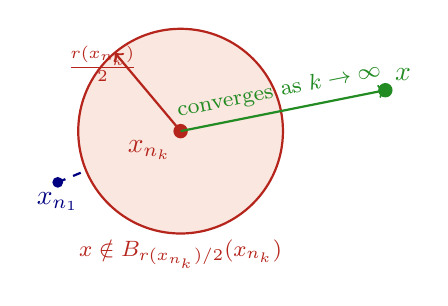
\begin{tikzpicture}[scale=1.3]
    % \begin{hidden}
    % - Canvas: scale=1.3, x-range [-0.5, 4.5], y-range [-0.8, 2.5]
    % - Elements: (1) Limit point x at (3.2, 1.2); (2) Subsequence points x_{n_k};
    %   (3) Convergent path arrow pointing to x; (4) Ball around x_{n_k} with x strictly outside;
    %   (5) Radius indicator r(x_{n_k})/2.
    % - Computations: Center of ball C = (1.2, 0.8), radius R = 1.0.
    %   Distance to x: d = sqrt((3.2-1.2)^2 + (1.2-0.8)^2) = sqrt(4 + 0.16) = sqrt(4.16) ≈ 2.04 > 1.0.
    %   Thus x is clearly outside the ball.
    % - Labels: x above right; x_{n_k} below left; ball label below.
    % - Collisions: None, elements well separated.
    % \end{hidden}
    \coordinate (X) at (3.2, 1.2);
    \coordinate (Xnk) at (1.2, 0.8);

    % Sequence points approaching x
    \fill[NavyBlue] (0.0, 0.3) circle (1.5pt) node[below] {$x_{n_1}$};
    \fill[NavyBlue] (0.6, 0.55) circle (1.5pt) node[below] {$x_{n_2}$};
    \draw[->, thick, dashed, NavyBlue] (0.0, 0.3) -- (0.6, 0.55);
    \draw[->, thick, dashed, NavyBlue] (0.6, 0.55) -- (Xnk);

    % Point x_{n_k} and its ball
    \draw[thick, BrickRed, fill=BrickRed!8] (Xnk) circle (1.0cm);
    \fill[BrickRed] (Xnk) circle (2pt) node[below left, BrickRed] {$x_{n_k}$};
    \draw[thick, BrickRed, ->] (Xnk) -- ++(130:1.0cm) node[midway, above left, font=\footnotesize] {$\frac{r(x_{n_k})}{2}$};

    % Limit point x
    \fill[ForestGreen] (X) circle (2pt) node[above right, ForestGreen, font=\bfseries] {$x$};
    \draw[->, thick, ForestGreen] (Xnk) -- (X) node[midway, above, sloped, font=\footnotesize] {converges as $k \to \infty$};
    \node[BrickRed, font=\footnotesize] at (1.2, -0.4) {$x \notin B_{r(x_{n_k})/2}(x_{n_k})$};
\end{tikzpicture}
\end{center}

Since $x_{n_k} \xrightarrow{k \to \infty} x$, the distance $d(x, x_{n_k})$ converges to $0$. By the squeeze principle applied to \eqref{eq:dist-lower-bound}:
\begin{equation}\label{eq:radius-goes-to-zero}
0 \le \frac{r(x_{n_k})}{2} \le d(x, x_{n_k}) \xrightarrow{k \to \infty} 0 \implies \lim_{k \to \infty} r(x_{n_k}) = 0.
\end{equation}
\end{content}

\begin{speech}[00:07:35 - 00:10:05]
And now that we know that this $r$ goes to zero, we will find easily a contradiction, because whatever is the $r$, $r$ of the limit point is a positive number, right? \inlinemetanote{writes $r(x) > 0$}

And then, since $x_{n_k}$ again is converging to $x$, \inlinemetanote{writes $x_{n_k} \to x$} eventually the ball of radius $r(x)/4$, centered at one of these points, $x_{n_k}$, is contained in the ball of radius $r(x)/2$, centered at $x$. \inlinemetanote{writes $B_{r(x)/4}(x_{n_k}) \subset B_{r(x)/2}(x) \subset U(x)$}

You see? The points are converging to here, and they are very, very close, and in this ball I have a lot of space: that is $r/4$ versus $r/2$. So, eventually --- you have the ball of radius $r/2$ is like this, and then I'm considering a point that is almost this one, this is the $x_{n_k}$, and the ball of radius $r/4$ is smaller ---, eventually this ball is inside of my bigger ball, right? Even if the center is slightly shifted.

And this, by definition, is contained in one of the open sets of the cover, right? But then this means that my choice of $r(x_{n_k})$ was not optimal; it was not respecting this, right? It was not the supremum. Because I'm saying that the ball of radius... remember that by optimality, or almost optimality, of $r(x_{n_k})$, \inlinemetanote{writes 'by optimality'} we should be able to take this $r(x_{n_k})$ as big as this number, right? As big as this number, yet we are saying that this goes to zero.

So, this is a contradiction, right? \inlinemetanote{writes 'is a contradiction' and draws a square}

This was the first implication, and I did it again because this is a hard proof. Not very long, but it's hard.
\end{speech}

\begin{content}[Deriving the Contradiction via Optimality of the Radius]
Since $x \in K$, \cref{eq:radius-function} guarantees that the limit point has a strictly positive radius:
\[
r(x) > 0.
\]
By convergence $x_{n_k} \xrightarrow{k \to \infty} x$, there exists an index $K_0 \in \mathbb{N}$ such that for all $k \ge K_0$:
\begin{equation}\label{eq:close-to-limit}
d(x_{n_k}, x) < \frac{r(x)}{4}.
\end{equation}

\textbf{Geometric Nesting of Balls:}
For any point $y \in B_{r(x)/4}(x_{n_k})$, the triangle inequality gives:
\[
d(y, x) \le d(y, x_{n_k}) + d(x_{n_k}, x) < \frac{r(x)}{4} + \frac{r(x)}{4} = \frac{r(x)}{2}.
\]
Therefore, the ball $B_{r(x)/4}(x_{n_k})$ is completely nested within $B_{r(x)/2}(x)$, which itself is contained in the assigned open set $U(x) \in \mathcal{U}$:
\begin{equation}\label{eq:nested-ball-inclusion}
B_{r(x)/4}(x_{n_k}) \subseteq B_{r(x)/2}(x) \subseteq U(x).
\end{equation}

\begin{center}
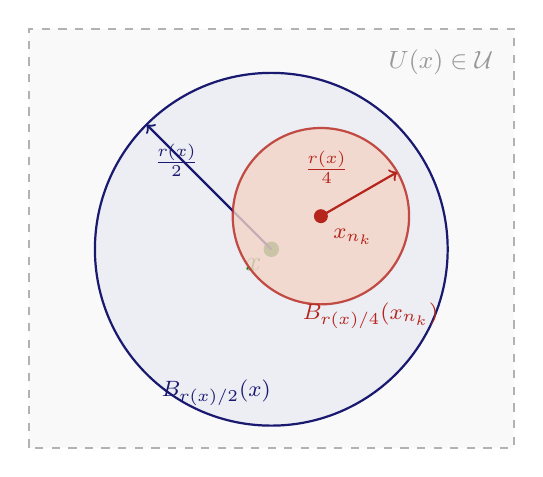
\begin{tikzpicture}[scale=1.4]
    % \begin{hidden}
    % - Canvas: scale=1.4, x in [-2.5, 2.5], y in [-2.2, 2.2]
    % - Elements: (1) Outer set U(x); (2) Big ball B_{r(x)/2}(x) around x;
    %   (3) Point x_{n_k} near x; (4) Small ball B_{r(x)/4}(x_{n_k}) nested inside the big ball.
    % - Computations: Center x at (0,0), radius R = 1.6.
    %   Point x_{n_k} at (0.45, 0.3), distance d = sqrt(0.45^2 + 0.3^2) ≈ 0.54 < 0.8 = R/2.
    %   Small ball radius r = 0.8. Max reach: 0.54 + 0.8 = 1.34 < 1.6 = R.
    %   Nesting is mathematically strict.
    % - Labels: x at (0,0); x_{n_k} at (0.45, 0.3); radii labeled on arrows.
    % \end{hidden}
    % Open set U(x) boundary
    \draw[thick, gray!60, fill=gray!5, dashed] (-2.2, -1.8) rectangle (2.2, 2.0);
    \node[gray!80, font=\small, anchor=north east] at (2.1, 1.9) {$U(x) \in \mathcal{U}$};

    % Big ball B_{r(x)/2}(x)
    \draw[thick, MidnightBlue, fill=MidnightBlue!8] (0,0) circle (1.6cm);
    \fill[ForestGreen] (0,0) circle (2pt) node[below left, ForestGreen] {$x$};
    \draw[->, thick, MidnightBlue] (0,0) -- (135:1.6cm) node[midway, above left, font=\footnotesize] {$\frac{r(x)}{2}$};

    % Small ball B_{r(x)/4}(x_{n_k})
    \coordinate (Xnk2) at (0.45, 0.3);
    \draw[thick, BrickRed, fill=BrickRed!15, opacity=0.8] (Xnk2) circle (0.8cm);
    \fill[BrickRed] (Xnk2) circle (1.8pt) node[below right=1pt, BrickRed, font=\footnotesize] {$x_{n_k}$};
    \draw[->, thick, BrickRed] (Xnk2) -- ++(30:0.8cm) node[midway, above left, font=\footnotesize] {$\frac{r(x)}{4}$};

    \node[MidnightBlue, font=\footnotesize] at (-0.5, -1.3) {$B_{r(x)/2}(x)$};
    \node[BrickRed, font=\footnotesize] at (0.9, -0.6) {$B_{r(x)/4}(x_{n_k})$};
\end{tikzpicture}
\end{center}

\textbf{Contradiction with Radius Vanishing:}
Since $B_{r(x)/4}(x_{n_k})$ is contained in $U(x) \in \mathcal{U}$, the definition of the supremum for $r(x_{n_k})$ implies:
\[
r(x_{n_k}) \ge \min \left\{ \frac{r(x)}{4}, \, 1 \right\} > 0 \quad \text{for all } k \ge K_0.
\]
In particular, $r(x_{n_k})$ is bounded below by the strictly positive constant $\min\{r(x)/4, 1\}$, which directly contradicts \cref{eq:radius-goes-to-zero}:
\[
\lim_{k \to \infty} r(x_{n_k}) = 0.
\]
This contradiction demonstrates that the sequence cannot be infinite; hence, the inductive construction must terminate after finitely many steps, yielding a finite subcover. Thus, sequential compactness implies topological compactness.
\end{content}

\subsection{Topological Compactness Implies Sequential Compactness (\texorpdfstring{$\mathbf{(2)} \implies \mathbf{(1)}$}{(2) => (1)})}

\begin{speech}[00:10:05 - 00:12:05]
The second one... \inlinemetanote{erases a line on the board and prepares the lower board}

Okay. The second one, \textbf{(2)} implies \textbf{(1)}, is slightly easier; it's a bit easier, right?

To show \textbf{(2)} implies \textbf{(1)}, we need to find... so, given... \inlinemetanote{writes 'Given $(x_n)_{n \ge 0} \subset K$ sequence'} given a sequence, our goal... \inlinemetanote{writes 'goal: show $\exists$ subsequence $(x_{n_k})$ convergent with limit in $K$'} our goal is to show that there exists a subsequence, that will be $x_{n_k}$, convergent, with limit in $K$, right?

And we will prove this again by contradiction. Assume that this does not happen. So, by contradiction... \inlinemetanote{writes 'by contradiction'}

Assume that this does not happen. Another way to put that is that for every $x$ in $K$, \inlinemetanote{writes '$\forall x \in K$, $x$ is not an accum. pt of $(x_n)$'} $x$ is not an accumulation point of my sequence.

Is this not an accumulation point? Remember that the definition of accumulation point is precisely that there is a subsequence that converges to $x$, right?
\end{speech}

\begin{content}[Proof Setup: Negation of Sequential Compactness]
We now prove the converse implication: assuming $K$ is topologically compact, we show that $K$ is sequentially compact.

\textbf{Setup:}
Let $(x_n)_{n \ge 0} \subseteq K$ be an arbitrary sequence in $K$.
\begin{align*}
\textbf{Goal:} &&& \text{Show that there exists a subsequence } (x_{n_k})_{k \ge 0} \text{ converging to some } x \in K.
\end{align*}

\textbf{Proof by Contradiction:}
Assume the contrary: no subsequence of $(x_n)$ converges to any point in $K$. That is:
\begin{equation}\label{eq:no-accumulation-point}
\forall x \in K, \quad x \text{ is not an accumulation point of } (x_n)_{n \ge 0}.
\end{equation}
\end{content}

\begin{speech}[00:12:05 - 00:14:00]
And now I will put it again in another form that is more suitable. So, what does it mean that $x$ is not an accumulation point?

I will claim, \inlinemetanote{writes 'claim:'} I will claim that this implies that for every $x$ in $K$, \inlinemetanote{writes '$\forall x \in K$'} there exists some $\varepsilon(x)$ positive \inlinemetanote{writes '$\exists \varepsilon(x) > 0$ such that'} such that my sequence... let me put it like this: my sequence $x_n$ visits \inlinemetanote{writes '$x_n$ visits $B_{\varepsilon(x)}(x)$ only finitely many times'} the ball of radius $\varepsilon(x)$ centered at $x$ only finitely many times.

The ball visits... well, let me put this in... this phrasing is easier to get intuition from, but what I mean mathematically is that $x_n$ belongs to the complement of this ball... so $x_n$ is always an element of... so, this is the same, right? \inlinemetanote{writes '$\iff x_n \in K \setminus B_{\varepsilon(x)}(x) \ \forall n \ge N(x)$'}

This is a way to say, if you want, that $x_n$ belongs to the complement of the ball for all $n$ bigger than or equal to a certain number that depends on $x$. Or eventually, all of the elements of the sequence will be in the complement of the ball. I'm saying the same in many equivalent ways. Is it clear?
\end{speech}

\begin{content}[Characterization via Finite Visits of Neighborhoods]
\begin{claim}\label[claim]{clm:finite-visits}
If $x \in K$ is not an accumulation point of $(x_n)_{n \ge 0}$, then there exists a radius $\varepsilon(x) > 0$ such that the sequence $(x_n)$ visits the open ball $B_{\varepsilon(x)}(x)$ only finitely many times. That is:
\begin{equation}\label{eq:finite-visits-formal}
\exists \varepsilon(x) > 0, \ \exists N(x) \in \mathbb{N} \quad \text{such that} \quad x_n \in K \setminus B_{\varepsilon(x)}(x) \quad \text{for all } n \ge N(x).
\end{equation}
\end{claim}
\end{content}

\begin{hidden}
% timestamp: 00:14:00
% topic: Proof of (2) => (1), claim that no accumulation point implies finite visits
% board_state: clm:finite-visits, eq:no-accumulation-point, eq:finite-visits-formal
% next_goal: Prove the claim by constructing a subsequence if it visited infinitely often, then build open cover
% open_loops: none
\end{hidden}

\begin{speech}[00:14:00 - 00:16:25]
So, why does $x$ not being an accumulation point imply this?

Well, because if... let's say, parenthesis, proof of claim: \inlinemetanote{writes '(proof of claim)'} if for every... let's say for $\varepsilon = 1/k$, so if for every $\varepsilon$ I can take $\varepsilon = 1/k$, and $k = 1$ to infinity, \inlinemetanote{writes 'if for $\varepsilon = 1/k$, $k = 1, \dots, \infty$'} $x_n$ visits infinitely many times the ball of radius $1/k$ centered at $x$, \inlinemetanote{writes '$x_n$ visits $\infty$-many times $B_{1/k}(x)$'} right?

Then I can pick a subsequence. I can say: okay, let me take $n_0$; I define it as $0$. \inlinemetanote{writes '$n_0 = 0$'} And then, since I always have infinitely many values, I will define $n_k$ always bigger than the previous one, or $n_{k+1}$ bigger than $n_k$, so that it is a subsequence, and such that $x_{n_{k+1}}$ is contained... let me put it like this to make it nicer: \inlinemetanote{writes '$n_k > n_{k-1}$ and $x_{n_k} \in B_{1/k}(x)$'} $n_k$ bigger than $n_{k-1}$ and $x_{n_k}$ is contained in the ball of radius $1/k$ centered at $x$.

You see? If you have infinitely many values, you can always pick one where the index is larger than the previous one, and it is going back to this ball. And this sequence would be a subsequence that converges to $x$. So, $x_{n_k}$ would converge to $x$ as $k$ goes to infinity. \inlinemetanote{writes 'So $x_{n_k} \to x$ as $k \to \infty$'}

Right? So, this is the proof of my claim. If I am assuming that no subsequence converges to $x$, no subsequence converging to $x$ necessarily implies that there is some $\varepsilon$ such that this ball is only visited finitely many times, okay?
\end{speech}

\begin{content}[Proof of the Finite-Visits Claim]
\begin{proof}[Proof of Claim \ref{clm:finite-visits}]
We argue by contraposition. Suppose that for every $\varepsilon > 0$, the sequence $(x_n)_{n \ge 0}$ visits $B_\varepsilon(x)$ infinitely many times.

Taking $\varepsilon_k = \frac{1}{k}$ for each $k \in \{1, 2, 3, \dots\}$, the set of indices $\{n \in \mathbb{N} \mid x_n \in B_{1/k}(x)\}$ is infinite. We can therefore construct a strictly increasing sequence of indices inductively:
\begin{itemize}
    \item Set $n_0 := 0$.
    \item For $k = 1$, pick $n_1 > n_0$ such that $x_{n_1} \in B_{1}(x)$.
    \item Having chosen $n_{k-1}$, since the ball $B_{1/k}(x)$ contains infinitely many terms of the sequence, pick an index $n_k > n_{k-1}$ such that:
    \[
    x_{n_k} \in B_{1/k}(x).
    \]
\end{itemize}
This defines a valid subsequence $(x_{n_k})_{k \ge 1}$. Furthermore, for every $k \ge 1$:
\[
d(x_{n_k}, x) < \frac{1}{k} \xrightarrow{k \to \infty} 0 \implies x_{n_k} \xrightarrow{k \to \infty} x.
\]
Thus, $(x_{n_k})$ is a subsequence of $(x_n)$ converging to $x \in K$, which means that $x$ is an accumulation point of $(x_n)$, contradicting our hypothesis \eqref{eq:no-accumulation-point}. This proves the claim.
\end{proof}
\end{content}

\begin{speech}[00:16:25 - 00:19:00]
And now with this, I can conclude, right? Because now I take the cover --- remember that now I want to use somewhere that my set is topologically compact, so I need to define a cover.

I define the cover $\mathcal{U}$... \inlinemetanote{writes '$\mathcal{U} = \{ B_{\varepsilon(x)}(x) \}_{x \in K}$'} You see that these are open balls, so they are in particular open sets, right? There are many of them, because $K$ could be very, very infinite... so in our examples in $\mathbb{R}$, this will be uncountable, many, many times. But okay, we have an arbitrary collection of balls, and now we can extract a finite subcover.

Then we can extract... since $K$ is topologically compact, \inlinemetanote{writes '$K$ top. cpt.'} there exists a finite subcover, so we can put $K \subset \bigcup_{j=1}^N B_{\varepsilon(y_j)}(y_j)$... \inlinemetanote{writes '$K \subset \bigcup_{j=1}^N B_{\varepsilon(y_j)}(y_j)$'}

Let me call the centers $y_j$, right? And now this is a contradiction. You see why?

Because any sequence has infinitely many terms. And I'm saying that my sequence would be visiting each of these balls finitely many times. But there are finitely many balls. So, at least one of the balls has to be visited infinitely many times. Contradiction!

So, this would imply that the sequence has finitely many terms, \inlinemetanote{writes 'this would imply seq has finitely many terms'} okay? Contradiction. \inlinemetanote{writes 'Contradiction $\square$'}
\end{speech}

\begin{content}[Deriving the Contradiction via Topological Compactness]
Using the radii $\varepsilon(x) > 0$ provided by Claim \ref{clm:finite-visits} for each $x \in K$, we construct the open cover:
\begin{equation}\label{eq:epsilon-cover}
\mathcal{U} := \bigl\{ B_{\varepsilon(x)}(x) \;\big|\; x \in K \bigr\}.
\end{equation}
Since each $B_{\varepsilon(x)}(x)$ is an open set containing $x$, $\mathcal{U}$ is indeed an open cover of $K$.

\textbf{Extracting a Finite Subcover:}
By the topological compactness of $K$, there exist finitely many points $y_1, \dots, y_N \in K$ such that:
\begin{equation}\label{eq:finite-subcover-balls}
K \subseteq \bigcup_{j=1}^N B_{\varepsilon(y_j)}(y_j).
\end{equation}

\textbf{Contradiction via the Pigeonhole Principle:}
\begin{itemize}
    \item By Claim \ref{clm:finite-visits}, for each $j \in \{1, \dots, N\}$, the sequence $(x_n)_{n \ge 0}$ visits $B_{\varepsilon(y_j)}(y_j)$ only finitely many times. That is, the set of indices:
    \[
    I_j := \bigl\{ n \in \mathbb{N} \;\big|\; x_n \in B_{\varepsilon(y_j)}(y_j) \bigr\}
    \]
    is finite for each $j \in \{1, \dots, N\}$.
    \item Since every term of the sequence lies in $K$ and $K \subseteq \bigcup_{j=1}^N B_{\varepsilon(y_j)}(y_j)$, we must have:
    \[
    \mathbb{N} = \bigcup_{j=1}^N I_j.
    \]
    \item A finite union of finite sets is finite, which implies that $\mathbb{N}$ is finite --- an immediate contradiction!
\end{itemize}
Therefore, at least one ball $B_{\varepsilon(y_j)}(y_j)$ must contain infinitely many terms of the sequence, contradicting Claim \ref{clm:finite-visits}.

Thus, the initial assumption \eqref{eq:no-accumulation-point} was false. Every sequence in $K$ possesses an accumulation point $x \in K$, which implies the existence of a convergent subsequence in $K$. Hence, $K$ is sequentially compact.
\end{content}

\end{proofWrapper}

\begin{speech}[00:19:00 - 00:20:50]
Okay. This is a difficult argument, I know. Now you have seen it. Maybe you have some questions about this, maybe not yet. We can also ask questions later on when you have them.

And then you can read it again... Last time, I also tried to draw pictures of the open sets and so on, so that you gain a bit of intuition, hopefully. And then you can read again the proof in the notes until it is clear. But this is, I know, a bit difficult.

So, the next thing, that will be easier, will be to... \inlinemetanote{erases the middle and lower boards and prepares to write consequences of compactness}
\end{speech}

\begin{note}[Board Transition]
The lecturer concludes the discussion of the equivalence between sequential and topological compactness, takes a brief moment for student questions, and thoroughly erases the lower and middle blackboard panels to introduce the corollaries of compactness.
\end{note}

\begin{hidden}
% timestamp: 00:20:50
% topic: Equivalence proof concluded; transitioning to consequences of compactness
% board_state: thm:compactness-equivalence
% next_goal: State and prove Corollaries 1, 2, and 3 (closedness, completeness, intersection)
% open_loops: none
\end{hidden}

\section{Corollaries of Compactness}

\begin{speech}[00:20:50 - 00:23:12]
Okay, so compact sets are very useful and very important. And now we will see some consequences, and you will start to... So, I think that some people are looking at the proof. Maybe is there some question?

\inlinemetanote{waits briefly for student questions; none are raised}

Okay, let me give some easier consequences of compactness: consequences, if you want, of the characterization of sequential compactness.

So, easy statements are, if you want, Corollary \textbf{1}: \inlinemetanote{writes 'Cor. 1'} for every metric space, if $K \subseteq X$ is compact, then $K$ is closed. \inlinemetanote{writes '$\forall (X, d)$ m.s. if $K \subset X$ cpt $\implies K$ is closed'}

Corollary \textbf{2} of sequential compactness: \inlinemetanote{writes 'Cor. 2'} if $K \subseteq X$ is compact, then $K$ is complete. \inlinemetanote{writes 'if $K \subset X$ cpt $\implies K$ is complete'}

And Corollary \textbf{3}: \inlinemetanote{writes 'Cor. 3'} if $K \subseteq X$ is compact and $A$ is closed, then the intersection of $K$ and $A$ is closed... sorry, closed, of course, but compact. \inlinemetanote{writes 'if $K \subset X$ cpt, $A \subset X$ closed $\implies K \cap A$ cpt'}
\end{speech}

\begin{content}[Fundamental Corollaries of Compactness]
Let $(X, d)$ be a metric space.

\begin{corollary}[Compact Subsets Are Closed]\label[corollary]{cor:compact-implies-closed}
If $K \subseteq X$ is compact, then $K$ is closed in $X$.
\end{corollary}

\begin{corollary}[Compact Subsets Are Complete]\label[corollary]{cor:compact-implies-complete}
If $K \subseteq X$ is compact, then $(K, d)$ is complete as a metric subspace.
\end{corollary}

\begin{corollary}[Intersection of Compact and Closed Subsets]\label[corollary]{cor:compact-closed-intersection}
If $K \subseteq X$ is compact and $A \subseteq X$ is closed, then $K \cap A$ is compact.
\end{corollary}

\begin{steps}[Overview of the Corollaries]
These three results provide immediate structural information about compact sets in arbitrary metric spaces:
\begin{itemize}
    \item \textbf{Closedness (\cref{cor:compact-implies-closed}):} Compact sets automatically contain all their limit points.
    \item \textbf{Completeness (\cref{cor:compact-implies-complete}):} Every Cauchy sequence in $K$ converges to a point in $K$, so compactness guarantees the absence of \qt{holes}.
    \item \textbf{Stability under Intersection (\cref{cor:compact-closed-intersection}):} Intersecting a compact set with a closed set retains compactness.
\end{itemize}
\end{steps}
\end{content}

\subsection{Proof of the Corollaries}

\begin{speech}[00:23:12 - 00:25:12]
These are all easy consequences of when you use this definition of compactness, for instance, sequential compactness, right? And what you know about the definitions of complete, closed, and so on and so forth.

So, I will say with words: each of them is a one-line proof using the definitions. But I will explain why this is true, and then it is a good... as always, you have everything in the notes, right? But you can do as an exercise: try to prove them, okay?

First thing: why is a compact set always closed? A compact subset is always closed. Well, you need to remember: compact subset with sequences is: every sequence has a convergent subsequence in the set. And we know also two characterizations of closed sets.

The first definition of a closed set was the complement of an open set. And then we saw also that a set is closed if and only if it contains the limits of convergent sequences. And this is the one we are going to use, right?

So, we will take any sequence in my compact set that is convergent, because we want to check that it is closed, right? Then it has a convergent subsequence, because it's compact, and the limit belongs to the set. And then, since the sequence is convergent, the full sequence converges to the same limit that is in my set, right?

If you understood as I said, it's clear and it's good for you. Otherwise, it's even better, because then it's a good opportunity to try to reproduce and do this proof by yourself.
\end{speech}

\begin{content}[Proof that Compact Subsets Are Closed]
\begin{proof}[Proof of Corollary \ref{cor:compact-implies-closed}]
We use the sequential characterization of closed sets: a subset $K \subseteq X$ is closed if and only if every convergent sequence in $K$ has its limit in $K$.

Let $(x_n)_{n \ge 0} \subseteq K$ be a sequence such that $x_n \xrightarrow{n \to \infty} x \in X$.
Since $K$ is compact (and therefore sequentially compact), there exists a subsequence $(x_{n_k})_{k \ge 0}$ that converges to some limit $y \in K$:
\[
x_{n_k} \xrightarrow{k \to \infty} y \in K.
\]
Because $(x_n)$ is already convergent to $x$ in $X$, every subsequence of $(x_n)$ must converge to the same limit. Thus, $y = x$. Since $y \in K$, we obtain $x \in K$. This proves that $K$ contains all its limit points, so $K$ is closed in $X$.
\end{proof}
\end{content}

\begin{speech}[00:25:12 - 00:27:12]
Corollary number \textbf{2}: if $K$ is compact, then it must be complete.

So, you take any Cauchy sequence. A Cauchy sequence is a sequence, so it will have a convergent subsequence in the set. And then, since it is Cauchy, every other subsequence will have the same limit, right? You need to show that; it's not difficult.

Again, Cauchy sequences are always about to converge. A Cauchy sequence is going to converge to some point. Just that sometimes, in some spaces, the limit point is not in my space, and I need to create it, like the rationals. A Cauchy sequence of rational numbers wants to converge; the problem is that maybe it wants to converge to the square root of $2$, and then it's not in my space. But compactness warrants that the limit is in the space, so no problem.

Corollary number \textbf{3}: if you have a compact set and you take a closed subset of my compact set --- so, for instance, you take $A$ closed ---, then this intersection is closed always, because the compact is closed, and $A$ is closed, and remember that the intersection of closed sets is closed, right? So, this intersection is closed. Then it is also compact. Again, sequential compactness: you just need to take a sequence in the intersection. In particular, the sequence is in $K$, so it has a convergent subsequence, and the limit is in $A$ because $A$ is closed, right?

So, we have these three consequences.
\end{speech}

\begin{content}[Proofs of Completeness and Closed Intersections]
\begin{proof}[Proof of Corollary \ref{cor:compact-implies-complete}]
Let $(x_n)_{n \ge 0} \subseteq K$ be a Cauchy sequence.
Since $K$ is sequentially compact, there exists a subsequence $(x_{n_k})_{k \ge 0}$ converging to some point $x \in K$.
A general property of Cauchy sequences in metric spaces states that if a Cauchy sequence possesses a subsequence converging to $x$, then the entire sequence converges to $x$:
\[
d(x_n, x) \le d(x_n, x_{n_k}) + d(x_{n_k}, x) \xrightarrow{n, k \to \infty} 0.
\]
Therefore, $(x_n)$ converges in $K$, proving that $(K, d)$ is complete.
\end{proof}

\begin{proof}[Proof of Corollary \ref{cor:compact-closed-intersection}]
Let $(x_n)_{n \ge 0} \subseteq K \cap A$ be an arbitrary sequence.
In particular, $(x_n) \subseteq K$. Since $K$ is sequentially compact, there exists a subsequence $(x_{n_k})_{k \ge 0}$ that converges to some limit $x \in K$.
At the same time, $(x_{n_k}) \subseteq A$. Since $A$ is closed, it contains all limits of its convergent sequences, whence $x \in A$.
Consequently, $x \in K \cap A$, which demonstrates that every sequence in $K \cap A$ has a convergent subsequence whose limit belongs to $K \cap A$. Thus, $K \cap A$ is compact.
\end{proof}
\end{content}

\begin{hidden}
% timestamp: 00:06:30
% topic: Corollaries of compactness (closedness, completeness, intersection with closed sets)
% board_state: cor:compact-implies-closed, cor:compact-implies-complete, cor:compact-closed-intersection
% next_goal: Proposition on continuous images of compact sets
% open_loops: none
\end{hidden}

\section{Continuous Images of Compact Sets}

\begin{speech}[00:27:13 - 00:29:41]
Something maybe slightly more interesting is the following proposition, but still easy, still easy. I don't remember if it is a proposition in the notes or a theorem... let me check... \inlinemetanote{checks lecture notes} I don't have it. Okay. Let's call it a proposition.

So, I will state it informally: a continuous image of a compact set is compact. \inlinemetanote{writes 'Prop (continuous image of cpt is cpt)'} This is the way you can remember the proposition: the continuous image of a compact set is always compact, right?

And now we phrase it a bit more precisely. So, $(X, d_X)$ is a metric space, as always, \inlinemetanote{writes '$(X, d_X)$ m.s.'} $K \subseteq X$ compact... \inlinemetanote{writes '$K \subset X$ cpt'} Well, let me put it: $(X, d_X)$ and $(Y, d_Y)$ are metric spaces, both, \inlinemetanote{writes '$(X, d_X), (Y, d_Y)$ m.s.'} and $f$ from $X$ to $Y$ is a continuous map, \inlinemetanote{writes '$f \colon X \to Y$ continuous'} and then, for every $K \subseteq X$ compact, \inlinemetanote{writes '$\forall K \subset X$ cpt'} $f(K)$ is also compact. \inlinemetanote{writes '$f(x) \subset Y$ cpt'} So, $f(K)$ is a subset of $Y$, right? \inlinemetanote{writes '$f(K) \subset Y$'}

And again, this is very, very useful; we will use this kind of thing many times. But it is very easy to prove when we have that, because, yeah...
\end{speech}

\begin{student}[Student Question]
You mean $f(K)$?
\end{student}

\begin{speech}[00:29:43 - 00:29:48]
Sorry? Yeah, exactly. \inlinemetanote{corrects $f(x)$ to $f(K)$ on the board} Thank you.
\end{speech}

\begin{speech}[00:29:48 - 00:32:15]
So, when you take a compact set and you compute the image by a continuous function, it is also compact.

How can we prove this? We can use either of the two definitions. With the sequential it is very easy; with the other, also. Let me do one of them. Which one? The sequential or the... let's see which one we use, right? Let's take number \textbf{2} to change a bit, right?

Okay. So, let's say that I want to show that the image is topologically compact, right? Goal: \inlinemetanote{writes 'Goal: show $f(K)$ top. cpt.'} show that $f(K)$ is topologically compact. So, this is the proof. I'm doing the proof of this proposition: Proof. \inlinemetanote{writes 'Proof'} My goal is to show that $f(K)$ is topologically compact.

So, you give me some open cover. Given $\mathcal{V}$ an open cover of $f(K)$, \inlinemetanote{writes 'given $\mathcal{V}$ open cover of $f(K)$'} there exists a finite subcover; this is what I want to show. I want to show that there exists a finite subcover. But what I can do with this open cover is to send it back by $f$ to an open cover of my set $K$.

So, given an open cover, I consider $\mathcal{U}$... \inlinemetanote{writes '$\mathcal{U} = \{ f^{-1}(V) \mid V \in \mathcal{V} \}$'} I hope you can see here... I consider calligraphic $\mathcal{U}$ to be the set of... let me put it like this: $f^{-1}(V)$, where $V$ belongs to my cover, right? And you see, I have my map $f$...
\end{speech}

\begin{speech}[00:32:15 - 00:34:26]
Here is the space $X$, \inlinemetanote{draws set $X$ on the board} right? Here is the space $Y$. \inlinemetanote{draws set $Y$ on the board} My map $f$ goes from here to here. \inlinemetanote{draws arrow $f \colon X \to Y$} And I have my compact set here, \inlinemetanote{draws set $K$ inside $X$} $K$. And this is $f(K)$, \inlinemetanote{draws image $f(K)$ inside $Y$} and I want to show that that is compact.

So, what I can take is some open cover here, \inlinemetanote{draws open cover $\mathcal{V}$ covering $f(K)$} right? I take my cover; this is $\mathcal{V}$. And remember that a function is continuous if and only if, when I map back open sets, it gives me open sets. And since those cover $f(K)$, when I compute the preimage of all these open sets, they cover $K$. \inlinemetanote{draws preimages covering $K$} So, these are the preimages of my sets, right?

Then this thing, being an open cover of $K$, will have a finite subcover. And now I will take the finitely many sets here, and I map them there; they are a finite subcover. End of the proof, okay?

So, extract a finite subcover, \inlinemetanote{writes 'extract finite subcover'} and then map it to the target: \inlinemetanote{writes 'and then map it to the target'} map it to the codomain. \inlinemetanote{writes 'map it to the codomain'} Put it here. Okay.

With sequential compactness it is very easy also. You use the definition of continuity with sequences, and it will be very easy, one line. Okay.
\end{speech}

\begin{content}[Continuous Image of Compact Sets and the Topological Proof]
\begin{proposition}[Continuous Image of a Compact Set]\label[proposition]{prop:continuous-image-compact}
Let $(X, d_X)$ and $(Y, d_Y)$ be metric spaces, and let $f \colon X \to Y$ be a continuous map.
If $K \subseteq X$ is compact, then its image $f(K) \subseteq Y$ is also compact.
\end{proposition}

\begin{proof}[Topological Proof (Using Open Covers)]
\textbf{Goal:} Show that $f(K)$ is topologically compact.

Let $\mathcal{V} = \{V_j\}_{j \in J}$ be an arbitrary open cover of $f(K)$ in $Y$, so that:
\[
f(K) \subseteq \bigcup_{j \in J} V_j.
\]
For each open set $V_j \in \mathcal{V}$, consider its preimage $f^{-1}(V_j) \subseteq X$. Since $f$ is continuous, the preimage of every open set in $Y$ is open in $X$.

We define the family of open sets in $X$:
\begin{equation}\label{eq:pullback-cover}
\mathcal{U} := \bigl\{ f^{-1}(V) \;\big|\; V \in \mathcal{V} \bigr\}.
\end{equation}
Since $f(K) \subseteq \bigcup_{j \in J} V_j$, taking preimages yields:
\[
K \subseteq f^{-1}(f(K)) \subseteq f^{-1}\left( \bigcup_{j \in J} V_j \right) = \bigcup_{j \in J} f^{-1}(V_j).
\]
Thus, $\mathcal{U}$ is an open cover of $K$.

Because $K$ is compact, it possesses a finite subcover: there exist finitely many indices $j_1, \dots, j_N \in J$ such that:
\begin{equation}\label{eq:finite-subcover-K}
K \subseteq \bigcup_{k=1}^N f^{-1}(V_{j_k}).
\end{equation}
Applying $f$ to both sides, we obtain:
\begin{equation}\label{eq:finite-subcover-fK}
f(K) \subseteq f\left( \bigcup_{k=1}^N f^{-1}(V_{j_k}) \right) = \bigcup_{k=1}^N f\bigl(f^{-1}(V_{j_k})\bigr) \subseteq \bigcup_{k=1}^N V_{j_k}.
\end{equation}
Therefore, $\{V_{j_1}, \dots, V_{j_N}\}$ is a finite subcover of $f(K)$ extracted from $\mathcal{V}$. Hence, $f(K)$ is topologically compact.
\end{proof}

\begin{center}
\begin{tikzpicture}[scale=1.15, >=Stealth]
% \begin{hidden}
% - Canvas: scale 1.15; space X centered at (-2.8, 0), space Y centered at (2.8, 0).
% - Order:
%   1. Outer domain blobs X and Y in dark gray outlines.
%   2. Mapping arrow f between X and Y at top with bend left=15.
%   3. Subsets K \subset X and f(K) \subset Y filled in BurntOrange!12 and outlined in BurntOrange.
%   4. Open cover V on the right covering f(K) in ForestGreen (dashed).
%   5. Pullback open cover U on the left covering K in ForestGreen (dashed).
%   6. Labels for X, Y, f, K, f(K), V, f^{-1}(V).
% - Coordinates:
%   X centered at (-2.8, 0), radii 2.0 and 1.4; Y centered at (2.8, 0), radii 2.0 and 1.4;
%   K centered at (-2.8, -0.1), radii 1.0 and 0.7; f(K) centered at (2.8, -0.1), radii 1.0 and 0.7;
%   Cover sets on right: V1 at (2.3, 0.25), V2 at (3.2, 0.2), V3 at (2.4, -0.35), V4 at (3.3, -0.3);
%   Cover sets on left: U1 at (-3.3, 0.25), U2 at (-2.4, 0.2), U3 at (-3.2, -0.35), U4 at (-2.3, -0.3).
% - Collisions: no labels intersect geometry.
% \end{hidden}
    % Space X
    \draw[thick, gray!80] (-2.8, 0) ellipse (2.0cm and 1.4cm);
    \node[anchor=south west, gray!90!black, font=\bfseries] at (-4.6, 1.0) {$X$};

    % Space Y
    \draw[thick, gray!80] (2.8, 0) ellipse (2.0cm and 1.4cm);
    \node[anchor=south east, gray!90!black, font=\bfseries] at (4.6, 1.0) {$Y$};

    % Mapping arrow f
    \draw[->, thick, MidnightBlue] (-0.8, 0.8) to[bend left=18] node[midway, above] {$f$} (0.8, 0.8);

    % Subset K
    \draw[thick, BurntOrange, fill=BurntOrange!12] (-2.8, -0.1) ellipse (1.0cm and 0.7cm);
    \node[BurntOrange!90!black, font=\bfseries] at (-2.8, -0.1) {$K$};

    % Subset f(K)
    \draw[thick, BurntOrange, fill=BurntOrange!12] (2.8, -0.1) ellipse (1.0cm and 0.7cm);
    \node[BurntOrange!90!black, font=\bfseries] at (2.8, -0.1) {$f(K)$};

    % Open cover V on the right (Y)
    \draw[dashed, ForestGreen, thick] (2.3, 0.25) ellipse (0.65cm and 0.45cm);
    \draw[dashed, ForestGreen, thick] (3.2, 0.2) ellipse (0.65cm and 0.45cm);
    \draw[dashed, ForestGreen, thick] (2.4, -0.35) ellipse (0.65cm and 0.45cm);
    \draw[dashed, ForestGreen, thick] (3.3, -0.3) ellipse (0.65cm and 0.45cm);
    \node[ForestGreen, font=\small] at (4.0, 0.5) {$\mathcal{V} = \{V_j\}$};

    % Pullback cover U on the left (X)
    \draw[dashed, ForestGreen, thick] (-3.3, 0.25) ellipse (0.65cm and 0.45cm);
    \draw[dashed, ForestGreen, thick] (-2.4, 0.2) ellipse (0.65cm and 0.45cm);
    \draw[dashed, ForestGreen, thick] (-3.2, -0.35) ellipse (0.65cm and 0.45cm);
    \draw[dashed, ForestGreen, thick] (-2.3, -0.3) ellipse (0.65cm and 0.45cm);
    \node[ForestGreen, font=\small] at (-4.2, -0.7) {$\mathcal{U} = \{f^{-1}(V_j)\}$};
\end{tikzpicture}
\end{center}

\begin{steps}[Sequential Alternative Proof]
As noted by the lecturer, the proposition also admits a very direct one-line proof using sequential compactness and sequential continuity:
\begin{enumerate}[label=\textbf{(\arabic*)}]
    \item Let $(y_n)_{n \ge 0} \subseteq f(K)$ be an arbitrary sequence. By definition of the image, there exists a sequence $(x_n)_{n \ge 0} \subseteq K$ such that $y_n = f(x_n)$ for all $n \ge 0$.
    \item Since $K$ is sequentially compact, $(x_n)$ has a subsequence $(x_{n_k})_{k \ge 0}$ converging to some $x \in K$.
    \item Since $f$ is continuous, it is sequentially continuous, so:
    \[
    y_{n_k} = f(x_{n_k}) \xrightarrow{k \to \infty} f(x) \in f(K).
    \]
    Thus, $(y_n)$ possesses a subsequence converging to a point in $f(K)$, which proves that $f(K)$ is sequentially compact.
\end{enumerate}
\end{steps}
\end{content}

\begin{hidden}
% timestamp: 00:13:45
% topic: Continuous image of a compact set is compact (Proposition & topological proof)
% board_state: prop:continuous-image-compact
% next_goal: Extreme Value Theorem for continuous functions on compact sets
% open_loops: none
\end{hidden}

\begin{speech}[00:34:26 - 00:35:43]
Further consequences of compactness, still in the abstract setup, is that continuous functions...

Where is the eraser? Ah, now I lost... \inlinemetanote{searches for the eraser} I lost the eraser, but I put it there, okay.

Many times we will consider real-valued functions on our space, that would be $\mathbb{R}^n$ or some other metric space, but most of the time $\mathbb{R}^n$.
\end{speech}

\section{The Extreme Value Theorem (Weierstrass Theorem)}

\begin{speech}[00:35:43 - 00:37:43]
So, we will consider maps from $X$ to $\mathbb{R}$ \inlinemetanote{writes 'Thm $f \colon X \to \mathbb{R}$ continuous'} continuous, many times. And then, on compact subsets, this map always attains the supremum and the infimum.

The supremum \inlinemetanote{writes '$\sup \{f(x) \mid x \in K\}$'} of $f(x)$ when $x$ in $K$ --- so $K$ is compact, \inlinemetanote{writes '$K \subset X$ cpt'} --- the supremum of $f(x)$ when $x$ in $K$, and the same with the infimum, \inlinemetanote{writes '$\inf$'} are attained. \inlinemetanote{writes 'are attained'}

Are attained means that there exists some $z$ in $K$ \inlinemetanote{writes '$\exists z \in K$'} --- are attained in $K$, right? \inlinemetanote{writes 'attained in $K$'} --- such that $f(z)$ is equal to the supremum, \inlinemetanote{writes '$f(z) = \sup$'} right? When we put it this way: the supremum when $x$ in $K$ of $f(x)$. \inlinemetanote{writes '$\sup_{x \in K} f(x)$'}

Are you familiar with this notation, supremum? It is the same, right? \inlinemetanote{circles $\sup \{f(x) \mid x \in K\}$ and points to $\sup_{x \in K} f(x)$} I can also put it like this, or with this below the supremum. It's notation.
\end{speech}

\begin{content}[The Extreme Value Theorem on Compact Metric Spaces]
\begin{theorem}[Extreme Value Theorem / Weierstrass Theorem]\label[theorem]{thm:weierstrass-extreme-value}
Let $(X, d)$ be a metric space, $K \subseteq X$ a compact subset, and $f \colon X \to \mathbb{R}$ a continuous function.
Then $f$ is bounded on $K$ and attains its supremum and infimum on $K$. That is, there exist points $z_{\max}, z_{\min} \in K$ such that:
\begin{equation}\label{eq:weierstrass-extrema}
f(z_{\max}) = \sup_{x \in K} f(x) \quad \text{and} \quad f(z_{\min}) = \inf_{x \in K} f(x).
\end{equation}
Equivalently:
\[
\min_{x \in K} f(x) = f(z_{\min}) \le f(x) \le f(z_{\max}) = \max_{x \in K} f(x) \quad \text{for all } x \in K.
\]
\end{theorem}
\end{content}

\begin{speech}[00:37:43 - 00:39:13]
Why is the supremum attained? And the infimum the same?

Well, you can see this in two ways. One way is I can use that... Okay, not yet, because I need to prove something, but let me do the second way, sorry. Later I will do a comment on how you can view this theorem when we have Heine--Borel.

We can prove this very easily using sequential compactness, right? By definition of the supremum, there exists some... if you call it $S$, the supremum... \inlinemetanote{writes '$S$'}

I will do it for the supremum, right? But the infimum is the same. If this supremum you call it $S$, \inlinemetanote{boxes $\sup \{f(x) \mid x \in K\}$ as $S$} by definition of supremum there exists some sequence \inlinemetanote{writes '$\exists (x_n) \subset K$'} $x_n$ such that $f(x_n)$ is converging to $S$, \inlinemetanote{writes '$f(x_n) \to S$'} right?
\end{speech}

\begin{speech}[00:39:13 - 00:40:25]
Actually, I can even take the sequence converging like that --- I mean, monotonely, right? So, I can even take $f(x_n)$ increasing or non-decreasing, \inlinemetanote{writes '($f(x_n)$ non-decreasing)'} if I want.

Maybe the supremum is not attained, but by definition of supremum there have to be points that are closer and closer in the image, right?

And then, this sequence, because $K$ is compact, has a convergent subsequence: \inlinemetanote{writes '$\exists x_{n_k} \to z \in K$'} there exists some $x_{n_k}$ converging to some $z$, right? And this belongs to $K$. But then, since $f$ is continuous, $f(z)$ is equal to $S$, \inlinemetanote{writes '$f(z) = S$'} so the supremum is attained.

So, this uses that $f$ is continuous, \inlinemetanote{writes '($f$ continuous)'} right? $f$ is sequentially continuous, so $f$ of the limit is equal to the limit of the $f$'s. $f$ of the limit is equal to that.
\end{speech}

\begin{speech}[00:40:25 - 00:41:13]
And the same applies to the infimum. The infimum is attained, and we call it minimum.

This you already saw in $\mathbb{R}$, right? In $\mathbb{R}$ you said: if you have a closed, bounded interval, the infimum and the supremum of a function are attained, and we call them minimum and maximum. But this is much more general; this applies to any compact space.
\end{speech}

\begin{content}[Proof of the Extreme Value Theorem via Sequential Compactness]
\begin{proof}[Proof of Theorem \ref{thm:weierstrass-extreme-value}]
We prove that the supremum is attained; the proof for the infimum is completely analogous.

Let $S := \sup_{x \in K} f(x) \in (-\infty, \infty]$. By the definition of the supremum, there exists a sequence of points $(x_n)_{n \ge 0} \subseteq K$ such that:
\begin{equation}\label{eq:optimizing-sequence}
f(x_n) \xrightarrow{n \to \infty} S.
\end{equation}
(Without loss of generality, we can choose $(x_n)$ such that the sequence of values $(f(x_n))_{n \ge 0}$ is monotonically non-decreasing).

Since $K$ is compact, it is sequentially compact. Therefore, $(x_n)$ has a subsequence $(x_{n_k})_{k \ge 0}$ that converges to some limit point $z \in K$:
\[
x_{n_k} \xrightarrow{k \to \infty} z \in K.
\]
Because $f$ is continuous, it is sequentially continuous. Hence:
\[
f(x_{n_k}) \xrightarrow{k \to \infty} f(z).
\]
On the other hand, $(f(x_{n_k}))_{k \ge 0}$ is a subsequence of the sequence $(f(x_n))_{n \ge 0}$ which converges to $S$. By the uniqueness of limits in $\mathbb{R}$:
\[
f(z) = S = \sup_{x \in K} f(x).
\]
Since $z \in K$, we have $f(z) \in \mathbb{R}$, which in particular implies that $S < \infty$ (so $f$ is bounded from above on $K$) and that the supremum is attained at $z \in K$.

Applying the exact same argument to $-f$ (or directly to $\inf_{x \in K} f(x)$), there exists a point $z_{\min} \in K$ such that $f(z_{\min}) = \inf_{x \in K} f(x) > -\infty$.
\end{proof}
\end{content}

\begin{hidden}
% timestamp: 00:20:30
% topic: Extreme Value Theorem (Weierstrass Theorem) on compact metric spaces
% board_state: thm:weierstrass-extreme-value
% next_goal: The Heine-Borel Theorem in \mathbb{R}^n
% open_loops: none
\end{hidden}

\section{The Heine--Borel Theorem in \texorpdfstring{$\mathbb{R}^n$}{R^n}}

\begin{speech}[00:41:13 - 00:43:13]
Now, all of this is in this huge level of generality. But we want to understand very, very well for this course the case of $\mathbb{R}^n$. \inlinemetanote{writes '$\mathbb{R}^n$'}

So, what happens in $\mathbb{R}^n$? In $\mathbb{R}^n$, we have a theorem that we will prove now, that is called Heine--Borel: \inlinemetanote{writes 'Thm (Heine-Borel)'} that says that $K \subseteq \mathbb{R}^n$ is compact \inlinemetanote{writes '$K \subset \mathbb{R}^n$ cpt'} if and only if $K$ is bounded and closed. \inlinemetanote{writes '$\iff K$ is bdd \& closed'} Right?

This equivalence only works for $\mathbb{R}^n$, not general metric spaces; in general metric spaces this is not true. But in $\mathbb{R}^n$, this is the case, and we will see a proof of that.

What does it mean that $K$ is bounded? You can give several equivalent definitions. One thing is that there exists some $N$ large \inlinemetanote{writes '$\exists N \in \mathbb{N}$ large'} --- you can take it integer --- such that the ball of radius $N$ centered at zero \inlinemetanote{writes '$B_N(0)$'} --- this is a ball in $\mathbb{R}^n$, right? \inlinemetanote{writes '$\subset \mathbb{R}^n$'} --- contains my set. \inlinemetanote{writes '$\supset K$'}

A bounded set you can put inside of a huge ball, right? On the contrary, a set is unbounded if it has a sequence of points... if this cannot exist, it means that it has a sequence of points that diverges to infinity in some direction, right?
\end{speech}

\begin{content}[The Heine--Borel Theorem and Boundedness in Euclidean Space]
\begin{theorem}[Heine--Borel Theorem in $\mathbb{R}^n$]\label[theorem]{thm:heine-borel}
Let $K \subseteq \mathbb{R}^n$ be equipped with the standard Euclidean metric. Then:
\begin{equation}\label{eq:heine-borel-equivalence}
K \text{ is compact} \iff K \text{ is closed and bounded}.
\end{equation}
\end{theorem}

\begin{definition}[Bounded Subset of $\mathbb{R}^n$]\label[definition]{def:bounded-set-rn}
A subset $K \subseteq \mathbb{R}^n$ is \newterm{bounded} if there exists $N \in \mathbb{N}$ such that $K$ is contained in the open ball of radius $N$ centered at the origin:
\begin{equation}\label{eq:bounded-ball}
K \subseteq B_N(0) = \bigl\{ x \in \mathbb{R}^n \;\big|\; \|x\| < N \bigr\}.
\end{equation}
\end{definition}

\begin{steps}[Heine--Borel As a Specific Euclidean Property]
The lecturer explicitly emphasizes that the equivalence between compactness and being \qt{closed and bounded} is a special feature of finite-dimensional Euclidean space $\mathbb{R}^n$:
\begin{itemize}
    \item In general metric spaces $(X, d)$, compactness always implies closedness and boundedness (\cref{cor:compact-implies-closed}), but the converse fails dramatically (for example, in infinite-dimensional normed spaces or in discrete metric spaces with infinitely many points, the unit ball is closed and bounded but not compact).
    \item In $\mathbb{R}^n$, the local geometry allows us to reduce compactness to boundedness and closedness via the Bolzano--Weierstrass theorem.
\end{itemize}
\end{steps}
\end{content}

\subsection{Metric Characterization of Boundedness}

\begin{speech}[00:43:13 - 00:44:52]
Another way to put the same --- you can prove that it's the same, and that is a bit more for any metric, whereas this is a bit more for $\mathbb{R}^n$ ---: if you want to define an unbounded set in a metric space, you can define that the supremum of the distance between $x$ and $x'$ \inlinemetanote{writes '$\sup_{x, x' \in K} d(x, x')$'} when $x$ and $x'$ belong to my set \inlinemetanote{writes '$x, x' \in K$'} is finite. Sorry, if it is finite, it is bounded; if it is infinite, it is unbounded.

This applies to any metric space. So, how can you say if a subset is very large in a metric space? You take any pair of points in your set and see if the distance grows more and more and more: the set has a very, very long diameter, right? And then it's unbounded.

After the break, we will prove this theorem. \inlinemetanote{writes 'Proof'}

So, proof...

Are you aware of the theorem of conservation of the syllabus, right? Are you aware of this theorem?

It's like the conservation of energy: the syllabus of the course is conserved, and what is not conserved is the pace at which I teach. So, if we lose time, I just will rush theorems, but I will teach the same, so...
\end{speech}

\begin{content}[Boundedness in General Metric Spaces]
\begin{definition}[Diameter and Metric Boundedness]\label[definition]{def:boundedness-diameter}
Let $(X, d)$ be a metric space. The \newterm{diameter} of a non-empty subset $K \subseteq X$ is defined by:
\begin{equation}\label{eq:set-diameter}
\operatorname{diam}(K) := \sup_{x, x' \in K} d(x, x') \in [0, \infty].
\end{equation}
A subset $K \subseteq X$ is called \newterm{bounded} if $\operatorname{diam}(K) < \infty$, and \newterm{unbounded} if $\operatorname{diam}(K) = \infty$.
\end{definition}

\begin{steps}[Equivalence of Boundedness Definitions in $\mathbb{R}^n$]
In $\mathbb{R}^n$, the ball-containment condition $K \subseteq B_N(0)$ and the finite-diameter condition $\operatorname{diam}(K) < \infty$ are equivalent:
\begin{itemize}
    \item If $K \subseteq B_N(0)$, then for all $x, x' \in K$, the triangle inequality gives $d(x, x') \le \|x\| + \|x'\| < 2N$, so $\operatorname{diam}(K) \le 2N < \infty$.
    \item Conversely, if $\operatorname{diam}(K) = D < \infty$, fixing any point $x_0 \in K$ gives $K \subseteq B_{D+1}(x_0)$. By setting $N := D + 1 + \|x_0\|$, we obtain $K \subseteq B_N(0)$.
\end{itemize}
\end{steps}
\end{content}

\begin{insight}[The \qt{Conservation of the Syllabus}]
The lecturer playfully presents the \qt{conservation of the syllabus} in analogy to the conservation of energy in physics: the material to be covered throughout the semester is constant and invariant. Consequently, if classroom pacing slows down, the velocity of lecturing must accelerate to conserve the total curriculum.
\end{insight}

\begin{proofWrapper}[Proof of Theorem \ref{thm:heine-borel}]

\subsection{Necessity: Compact Subsets Are Closed and Bounded (\texorpdfstring{$\implies$}{=>})}

\begin{speech}[00:44:52 - 00:46:48]
Proof: we need to show... there is an easy implication.

If $K$ in $\mathbb{R}^n$ is compact, I want to show that $K$ is... well, that $K$ is closed, I already showed, because this is a general property. So, by one of the corollaries, $K$ is closed, \inlinemetanote{writes '$\implies 1) \ K$ closed \checkmark'} because every compact set is closed, so this is okay.

And then, I want to show that $K$ is bounded... \inlinemetanote{writes '$2) \ K$ bdd'} Bounded --- this means bounded. \inlinemetanote{rewrites 'bounded'} That $K$ is bounded.

So, how do I show this? Okay, if $K$ were unbounded... \inlinemetanote{writes 'if $K$ were unbounded'} there exists some sequence... \inlinemetanote{writes '$\exists x_n$'}

Remember, the definition of bounded is this, right? \inlinemetanote{points at $B_N(0) \supset K$} So, if I say that $K$ is not bounded, it means that there is a sequence of capital $N$'s, if you want, \inlinemetanote{writes '$\exists (x_N)_{N \in \mathbb{N}} \subset K$'} such that the modulus of $x_N$ --- this is contained in $K$ --- is bigger than $N$ \inlinemetanote{writes '$|x_N| > N$'} for all $N$, \inlinemetanote{writes '$\forall N$'} right? I'm just using this definition of bounded.
\end{speech}

\begin{content}[Forward Direction: Closedness and Setup for Boundedness]
We prove the forward implication ($\implies$): assume $K \subseteq \mathbb{R}^n$ is compact.

\textbf{1. $K$ is closed:}
By Corollary \ref{cor:compact-implies-closed}, any compact subset of an arbitrary metric space is closed. Since $(\mathbb{R}^n, d_{\text{Euclidean}})$ is a metric space, $K$ is closed.

\textbf{2. $K$ is bounded (Proof by Contradiction):}
Suppose that $K$ were unbounded.
By \cref{def:bounded-set-rn}, $K \not\subseteq B_N(0)$ for any $N \in \mathbb{N}$. Therefore, for each $N \in \mathbb{N}$, there exists an element $x_N \in K$ such that:
\begin{equation}\label{eq:unbounded-sequence-norm}
x_N \in K \quad \text{and} \quad \|x_N\| > N.
\end{equation}
This constructs a sequence $(x_N)_{N \in \mathbb{N}} \subseteq K$ whose norms grow beyond all bounds.
\end{content}

\begin{speech}[00:46:48 - 00:48:31]
So, if it is not bounded, I can have a divergent sequence. And now you know that any subsequence of that cannot converge. So, any subsequence will diverge. \inlinemetanote{writes 'any subsequence will diverge'}

Indeed, \inlinemetanote{writes 'Indeed'} if I had some $x_{n_k}$ converging to $x$, \inlinemetanote{writes '$x_{n_k} \to x$'} because the modulus... or by the triangle inequality, right? I know that this is equivalent to $x_{n_k} - x$ converging to zero \inlinemetanote{writes '$|x_{n_k} - x| \to 0$'} as $k$ goes to infinity. \inlinemetanote{writes 'as $k \to \infty$'} But then I would have, by the triangle inequality, that $|x_{n_k}|$ \inlinemetanote{writes '$|x_{n_k}| \le$'} is less than or equal to this plus this: \inlinemetanote{writes '$|x_{n_k} - x| + |x|$'} this is the triangle inequality. Triangle, right? \inlinemetanote{writes 'triangle'}

And this is going to zero, and this is a bounded number, so this contradicts that, right? \inlinemetanote{points at $|x_N| > N$}

So, any compact set must be bounded in $\mathbb{R}^n$. \inlinemetanote{writes 'This shows $\implies$'}
\end{speech}

\begin{hidden}
% timestamp: 00:06:50
% topic: Heine-Borel Theorem in R^n (necessity proof)
% board_state: thm:heine-borel, def:bounded-subset-rn, eq:unbounded-sequence-norm
% next_goal: Transition to sufficiency direction (closed and bounded implies compact)
% open_loops: none
\end{hidden}

\begin{content}[Forward Direction: Deducing Boundedness via Divergence of Subsequences]
\textbf{Deriving the Contradiction:}
Since $K$ is compact, it is sequentially compact (\cref{thm:compactness-equivalence}). Therefore, the sequence $(x_N)_{N \in \mathbb{N}} \subseteq K$ must possess a convergent subsequence $(x_{N_k})_{k \in \mathbb{N}}$ converging to some limit point $x \in K$:
\[
x_{N_k} \xrightarrow{k \to \infty} x \in K \iff \|x_{N_k} - x\| \xrightarrow{k \to \infty} 0.
\]
By the reverse triangle inequality in $\mathbb{R}^n$:
\begin{equation}\label{eq:triangle-norm-bound}
\|x_{N_k}\| \le \|x_{N_k} - x\| + \|x\|.
\end{equation}
As $k \to \infty$, the term $\|x_{N_k} - x\|$ converges to $0$, and $\|x\|$ is a fixed constant. Thus, the sequence of norms $(\|x_{N_k}\|)_{k \in \mathbb{N}}$ must be bounded:
\[
\limsup_{k \to \infty} \|x_{N_k}\| \le \|x\| < \infty.
\]
However, by construction in \eqref{eq:unbounded-sequence-norm}, we have:
\[
\|x_{N_k}\| > N_k \ge k \xrightarrow{k \to \infty} \infty,
\]
which implies $\|x_{N_k}\| \to \infty$, an immediate contradiction!

Hence, our assumption was false: $K$ cannot be unbounded. Every compact subset $K \subseteq \mathbb{R}^n$ is necessarily bounded and closed. This completes the forward direction ($\implies$).
\end{content}

\subsection{Sufficiency: Closed and Bounded Subsets Are Compact (\texorpdfstring{$\Longleftarrow$}{<=})}

\begin{speech}[00:48:31 - 00:49:26]
And now we need to prove the hard work, that is the other implication. \inlinemetanote{shifts blackboards}

But... no. Now I'm looking at my notes because I always have the same problem: I remember the theorems, but I never remember the name of the theorem.

And how is this... now you can help me: what is the name of this theorem in $\mathbb{R}$, that when you have a sequence in a closed, bounded interval, there exists a convergent subsequence?
\end{speech}

\begin{student}[Student Answer]
Bolzano-Weierstrass.
\end{student}

\begin{speech}[00:49:28 - 00:50:04]
Ah, this! Thank you. Bolzano--Weierstrass.

Thank you. She said: Bolzano--Weierstrass. Thank you, this was what I was missing.

So, to prove Heine--Borel for $\mathbb{R}^n$, our proof will be based on Bolzano--Weierstrass for $\mathbb{R}$, right? We'll see how to use this property that you proved in Analysis 1 on each of the components of my sequence to extract a convergent subsequence.
\end{speech}

\begin{note}[Board Transition]
The lecturer thoroughly erases the lower blackboard panel in silence to prepare for the proof of the reverse implication ($\Longleftarrow$) of the Heine--Borel theorem.
\end{note}

\subsubsection{Reduction to Compactness of Closed Cubes}

\begin{speech}[00:50:58 - 00:52:33]
Heine--Borel, the difficult implication: that one. \inlinemetanote{writes '$\Longleftarrow$'} Right?

Our goal will be to show that, given $N$ in $\mathbb{N}$... \inlinemetanote{writes 'given $N \in \mathbb{N}$'} --- let's say, it's not important, given any number --- the cube $[-N, N]^n$, \inlinemetanote{writes '$[-N, N]^n \subset \mathbb{R}^n$'} the cube in $\mathbb{R}^n$, is compact, right? \inlinemetanote{writes 'is cpt'}

Why is this sufficient? This is sufficient \inlinemetanote{writes 'This is sufficient'} because then, if $K \subset \mathbb{R}^n$ \inlinemetanote{writes 'if $K \subset \mathbb{R}^n$'} is closed and bounded... \inlinemetanote{writes 'closed \& bdd'} Well, because it's bounded, we'll have that $K$ is contained in the ball of radius $N$ centered at zero, \inlinemetanote{writes '$K \subset B_N(0)$'} and the ball of radius $N$ is always contained in the cube, right? \inlinemetanote{writes '$\subset [-N, N]^n$'}
\end{speech}

\begin{speech}[00:52:33 - 00:54:20]
So, if you want, this is a simple exercise --- a nice property of the Euclidean distance. \inlinemetanote{writes 'Exercise: Euclidean distance'}

In the plane, you know this very well, but you can show this as an exercise in any dimension. So, you have the ball of radius $N$ is like that, right? \inlinemetanote{draws a circle on the board} And then the cube --- this cube of diameter $2N$ --- is bigger, contains the ball. \inlinemetanote{draws a square around the circle} It's tangent, actually, here, right? So, the ball is contained in the cube.

In any case, the important thing is that we'll have a closed subset of a compact set. So, if we prove that this is compact, $K$ will be a closed subset of a compact set, and then, by one of the corollaries of sequential compactness, this will also be compact. Since a closed subset of a compact set is compact, \inlinemetanote{writes '(closed subset of cpt is cpt)'} this will imply that $K$ is compact. \inlinemetanote{writes '$\implies K$ is cpt'}

So, we only need to show that the closed cubes like that --- these guys, \inlinemetanote{points at $[-N, N]^n$} for any $N$ given --- are compact sets. This is our goal, and this is what I will show now.
\end{speech}

\begin{content}[Sufficiency Strategy: Reducing to the Compactness of Cubes]
We prove the reverse implication ($\Longleftarrow$): assume $K \subseteq \mathbb{R}^n$ is closed and bounded.

\begin{lemma}[Compactness of Closed Cubes in $\mathbb{R}^n$]\label[lemma]{lem:cubes-compact}
For every $N \in \mathbb{N}$, the closed cube:
\begin{equation}\label{eq:cube-def}
Q_N := [-N, N]^n = \underbrace{[-N, N] \times [-N, N] \times \dots \times [-N, N]}_{n \text{ times}} \subset \mathbb{R}^n
\end{equation}
is compact in $(\mathbb{R}^n, d_{\text{Euclidean}})$.
\end{lemma}

\textbf{Proof that Lemma \ref{lem:cubes-compact} Implies the Reverse Implication:}
\begin{enumerate}[label=\textbf{(\arabic*)}]
    \item Since $K$ is bounded, by \cref{def:bounded-set-rn} there exists $N \in \mathbb{N}$ such that $K \subseteq B_N(0)$.
    \item Any point $x = (x_1, \dots, x_n) \in B_N(0)$ satisfies:
    \[
    \|x\|^2 = \sum_{j=1}^n x_j^2 < N^2 \implies |x_j| \le \sqrt{\sum_{j=1}^n x_j^2} < N \quad \text{for all } j \in \{1, \dots, n\}.
    \]
    Thus, $x_j \in [-N, N]$ for all $j \in \{1, \dots, n\}$, which gives the inclusion:
    \begin{equation}\label{eq:ball-in-cube}
    B_N(0) \subseteq [-N, N]^n.
    \end{equation}
    Consequently, $K \subseteq B_N(0) \subseteq Q_N$.
    \item Therefore, $K$ can be written as:
    \[
    K = K \cap Q_N.
    \]
    Since $K$ is closed in $\mathbb{R}^n$ by hypothesis, and $Q_N$ is compact by \cref{lem:cubes-compact}, \cref{cor:compact-closed-intersection} implies directly that $K = K \cap Q_N$ is compact!
\end{enumerate}

\begin{exercise}[Inclusion of Euclidean Ball in Cube]\label[exercise]{ex:euclidean-ball-in-cube}
Show that for all $N > 0$ and any dimension $n \ge 1$, the Euclidean ball $B_N(0) \subset \mathbb{R}^n$ is contained in the closed cube $[-N, N]^n$.
\end{exercise}

\begin{center}
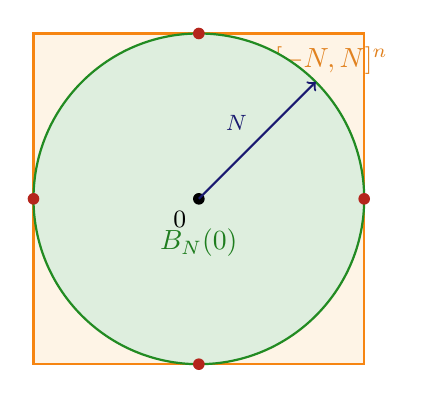
\begin{tikzpicture}[scale=1.4]
% \begin{hidden}
% - Canvas: scale 1.4; origin at (0,0); square [-N, N]^2 from (-1.5, -1.5) to (1.5, 1.5);
%   inscribed circle of radius 1.5.
% - Order: (1) shaded square [-N, N]^2 in BurntOrange!8 with BurntOrange border;
%   (2) Euclidean ball B_N(0) in ForestGreen!15 fill with ForestGreen border;
%   (3) tangent contact points; (4) radius arrow N; (5) labels.
% - Coordinates: square corners at (+-1.5, +-1.5), circle radius 1.5.
% - Labels: B_N(0) inside circle, [-N, N]^n in top right corner.
% \end{hidden}
    % Cube [-N, N]^n (illustrated in 2D)
    \draw[thick, BurntOrange, fill=BurntOrange!8] (-1.5, -1.5) rectangle (1.5, 1.5);
    \node[BurntOrange!90!black, font=\bfseries] at (1.2, 1.25) {$[-N, N]^n$};

    % Inscribed Ball B_N(0)
    \draw[thick, ForestGreen, fill=ForestGreen!15] (0,0) circle (1.5cm);
    \node[ForestGreen!90!black, font=\bfseries] at (0, -0.4) {$B_N(0)$};

    % Origin and Radius Vector
    \fill[black] (0,0) circle (1.5pt) node[below left=1pt, font=\small] {$0$};
    \draw[->, thick, MidnightBlue] (0,0) -- (45:1.5cm) node[midway, above left, font=\footnotesize] {$N$};

    % Tangent Points
    \fill[BrickRed] (1.5, 0) circle (1.5pt);
    \fill[BrickRed] (-1.5, 0) circle (1.5pt);
    \fill[BrickRed] (0, 1.5) circle (1.5pt);
    \fill[BrickRed] (0, -1.5) circle (1.5pt);
\end{tikzpicture}
\end{center}
\end{content}

\subsubsection{Componentwise Extraction via the Bolzano--Weierstrass Theorem}

\begin{speech}[00:54:20 - 00:56:36]
And to prove this, the proof reduces to Bolzano--Weierstrass in $\mathbb{R}$. \inlinemetanote{writes 'Proof reduces to Bolzano-Weierstrass in $\mathbb{R}$'}

The key is: how do we reduce from this theorem in $\mathbb{R}^n$ to something in $\mathbb{R}$? The idea is to pass to the components of my sequence.

Given a sequence $x_k$ in the cube, \inlinemetanote{writes '$(x_k) \subset [-N, N]^n$'} recall that for such a sequence we have the sequence of the components: we can write $x_k = (x_k^{(1)}, \dots, x_k^{(n)})$, \inlinemetanote{writes '$x_k = (x_k^{(1)}, \dots, x_k^{(n)})$'} the $n$ components of my vector.

And each of these is a sequence in $[-N, N]$. So, when I look at one of the components, it is a sequence in a closed and bounded interval of $\mathbb{R}$. So, I can apply Bolzano--Weierstrass to each of them, right?

To make one of the components converge is always easy --- well, you need to apply Bolzano--Weierstrass, but you can make one of the components converge. And now the trick is that I will extract a subsequence, and then a subsequence of the subsequence, and then a subsequence of the subsequence of the subsequence, and so on, finitely many times, until I get all the $n$ components to converge at the same time, okay?

Let's start with the first. First, I look at the first component.
\end{speech}

\begin{hidden}
% timestamp: 00:13:30
% topic: Reduction of Heine-Borel to compactness of cubes via Bolzano-Weierstrass
% board_state: lem:cubes-compact, ex:euclidean-ball-in-cube, eq:ball-in-cube
% next_goal: Inductive subsequence extraction across all n coordinate components
% open_loops: none
\end{hidden}

\begin{content}[Proof of Lemma \ref{lem:cubes-compact}: Component Decomposition]
\textbf{Proof of Lemma \ref{lem:cubes-compact} (Compactness of Closed Cubes):}

To prove that $Q_N = [-N, N]^n$ is compact, by \cref{thm:compactness-equivalence} it suffices to show that $Q_N$ is \textbf{sequentially compact}.

Let $(x_k)_{k \ge 0} \subseteq Q_N$ be an arbitrary sequence of points in the cube.
Each point $x_k \in \mathbb{R}^n$ decomposes into its $n$ coordinate components:
\begin{equation}\label{eq:vector-components}
x_k = \left( x_k^{(1)}, x_k^{(2)}, \dots, x_k^{(n)} \right) \in \mathbb{R}^n.
\end{equation}
Since $x_k \in Q_N = [-N, N]^n$, each individual coordinate sequence $(x_k^{(j)})_{k \ge 0}$ is a sequence of real numbers bounded in the compact interval $[-N, N] \subset \mathbb{R}$:
\[
x_k^{(j)} \in [-N, N] \quad \text{for all } k \ge 0 \text{ and all } j \in \{1, \dots, n\}.
\]
\end{content}

\begin{speech}[00:56:36 - 00:59:08]
\textbf{1}: \inlinemetanote{writes '1. Look at sequence'} look at the sequence $(x_k^{(1)})_{k \ge 0}$, \inlinemetanote{writes '$(x_k^{(1)})_{k \ge 0}$'} the first component, $k \ge 0$. This is a sequence in $[-N, N]$, \inlinemetanote{writes '$\subset [-N, N]$'} a sequence of real numbers. By Bolzano--Weierstrass, \inlinemetanote{writes 'by BW'} it has a convergent subsequence.

Let me put it like this, because there will be many subsequences, so I will need a more or less efficient notation for a subsequence of a subsequence. I will take some $k_1(m)$ \inlinemetanote{writes '$(x_{k_1(m)}^{(1)})_{m \ge 0}$'} --- this will be some increasing sequence in $\mathbb{N}$, \inlinemetanote{writes 'increasing sequence in $\mathbb{N}$'} a sequence of indices, and I call it $k_1$ because there will be more, right? --- such that the subsequence $x_{k_1(m)}^{(1)}$ converges to some limit that I call $L_1$. \inlinemetanote{writes '$\to L_1 \in [-N, N]$'}

This is an accumulation point of the first component, right?

So, I'm applying Bolzano--Weierstrass to that sequence of numbers, and then I am inferring the existence of a subsequence. This is how I call the indices of this subsequence, right? There is a sequence of increasing indices, and the first component converges to some number $L_1$, right?
\end{speech}

\begin{content}[Step 1: Convergent Subsequence for the First Coordinate Component]
\textbf{Step 1 (First Component):}
Consider the real-valued sequence of first coordinates:
\[
\bigl( x_k^{(1)} \bigr)_{k \ge 0} \subseteq [-N, N] \subset \mathbb{R}.
\]
Since $[-N, N]$ is a closed bounded interval in $\mathbb{R}$, by the 1-dimensional \textbf{Bolzano--Weierstrass theorem}, there exists a strictly increasing sequence of indices:
\[
k_1 \colon \mathbb{N} \to \mathbb{N}, \quad m \mapsto k_1(m) \quad \text{with } k_1(0) < k_1(1) < k_1(2) < \dots
\]
such that the corresponding subsequence of first components converges to some limit $L_1 \in [-N, N]$:
\begin{equation}\label{eq:first-component-limit}
\lim_{m \to \infty} x_{k_1(m)}^{(1)} = L_1 \in [-N, N].
\end{equation}
\end{content}

\begin{speech}[00:59:08 - 01:01:08]
Second step. \inlinemetanote{writes '2.'}

Now I look at the sequence of second components along this subsequence: \inlinemetanote{writes 'Look at'} $(x_{k_1(m)}^{(2)})_{m \ge 0}$. \inlinemetanote{writes '$(x_{k_1(m)}^{(2)})_{m \ge 0}$'} This is a different sequence, because here I had the first component. This is associated to the same subsequence of indices, right? I just look at what happens in the second component. And maybe this one is not converging --- because I can guarantee that the first component is converging, but the second maybe not.

But then, since this is contained in $[-N, N]$, \inlinemetanote{writes '$\subset [-N, N]$'} again, this is a compact set in $\mathbb{R}$, so by Bolzano--Weierstrass there exists a convergent subsequence.

This implies, again using Bolzano--Weierstrass a second time, \inlinemetanote{writes '$\implies$ by BW'} that there exists a second sequence of indices that I will call $k_2(m)$, \inlinemetanote{writes '$\exists (k_2(m))_{m \ge 0}$'} that is a subsequence of $k_1(m)$, \inlinemetanote{writes 'subsequence of $k_1(m)$'} such that $x_{k_2(m)}^{(2)}$ --- the second component now --- converges to some number $L_2$; \inlinemetanote{writes '$x_{k_2(m)}^{(2)}$'} I call $L_2$ the limit. \inlinemetanote{writes '$\to L_2$'} And this number belongs to $[-N, N]$. \inlinemetanote{writes '$\in [-N, N]$'}
\end{speech}

\begin{speech}[01:01:08 - 01:02:36]
Now, since this is a subsequence of the previous one, the first component, when I look along this subsequence, also converges to $L_1$. So, also $x_{k_2(m)}^{(1)}$ converges to $L_1$ as $m \to \infty$ --- I emphasize. \inlinemetanote{writes 'also $x_{k_2(m)}^{(1)} \to L_1$'}

Remember this lemma that I said was a bit silly, but that confused me and I gave a wrong statement last Wednesday? This is the correct one, so I'm using the correct one: when you have any sequence that converges to a limit, and you take a subsequence, it will still converge to the same limit. I'm just using that.

And then you continue! You will do this process as many times as components you have. Every time, you extract a subsequence of the previous subsequence, and every time, you make a new component converge. And since you have finitely many components, eventually all of the components converge.
\end{speech}

\begin{hidden}
% timestamp: 00:20:45
% topic: Subsequence of subsequence extraction for coordinate convergence
% board_state: eq:first-component-limit, eq:second-component-limit
% next_goal: Inductive step n, definition of limit point x = (L_1, ..., L_n)
% open_loops: none
\end{hidden}

\begin{content}[Step 2: Subsequence of the Subsequence for Simultaneous Convergence]
\textbf{Step 2 (Second Component):}
Now consider the sequence of second coordinates restricted to the index subsequence $k_1(m)$:
\[
\bigl( x_{k_1(m)}^{(2)} \bigr)_{m \ge 0} \subseteq [-N, N].
\]
While this sequence is not guaranteed to converge on its own, it is a bounded sequence in $[-N, N] \subset \mathbb{R}$. Applying the Bolzano--Weierstrass theorem a second time, there exists a strictly increasing subsequence of indices:
\[
k_2(m) = k_1(\ell(m)) \quad \text{such that } (k_2(m))_{m \ge 0} \text{ is a subsequence of } (k_1(m))_{m \ge 0},
\]
for which the second component converges to some limit $L_2 \in [-N, N]$:
\begin{equation}\label{eq:second-component-limit}
\lim_{m \to \infty} x_{k_2(m)}^{(2)} = L_2 \in [-N, N].
\end{equation}

\textbf{Simultaneous Convergence of the First Two Components:}
Crucially, because $(k_2(m))_{m \ge 0}$ is a subsequence of $(k_1(m))_{m \ge 0}$, and every subsequence of a convergent sequence converges to the same limit, the first component also converges along $(k_2(m))$ to $L_1$:
\[
\lim_{m \to \infty} x_{k_2(m)}^{(1)} = L_1 \in [-N, N].
\]
Thus, along the single subsequence of indices $(k_2(m))_{m \ge 0}$, \textbf{both} the first and second components converge simultaneously to $(L_1, L_2) \in [-N, N]^2$.
\end{content}

\begin{note}[Board Transition]
The lecturer erases the bottom-left panel of the blackboard to make room for writing the general inductive step ($n$ components) and assembling the limit vector.
\end{note}

\begin{speech}[01:03:34 - 01:05:21]
Continuing this process... \inlinemetanote{writes 'Continuing this process'}

We need to repeat this process $n$ times, because we have $n$ components, right? Until we get a last subsequence, $(k_n(m))_{m \ge 0}$, \inlinemetanote{writes '$(k_n(m))_{m \ge 0}$'} $m \ge 0$, right?

And then, for this subsequence, we will have $x_{k_n(m)}^{(n)}$... \inlinemetanote{writes '$x_{k_n(m)}^{(n)}$'} as $m$ goes to infinity, this will converge to some number $L_n$ \inlinemetanote{writes '$\xrightarrow{m \to \infty} L_n$'} that is in $[-N, N]$, right? \inlinemetanote{writes '$\in [-N, N]$'}

And also, because it's a subsequence of the subsequence of the subsequence of all the previous ones, $x_{k_n(m)}^{(j)}$ --- any other component $j$ --- also converges to $L_j$ \inlinemetanote{writes '$x_{k_n(m)}^{(j)} \to L_j$'} from previous steps, right? \inlinemetanote{writes 'from previous steps'}
\end{speech}

\begin{content}[Inductive Step for All \texorpdfstring{$n$}{n} Coordinate Components]
By iterating this extraction process $n$ times, we obtain a nested chain of index subsequences:
\[
(k_n(m))_{m \ge 0} \subseteq (k_{n-1}(m))_{m \ge 0} \subseteq \dots \subseteq (k_1(m))_{m \ge 0} \subseteq \mathbb{N},
\]
such that for the final coordinate $n$:
\begin{equation}\label{eq:nth-component-limit}
\lim_{m \to \infty} x_{k_n(m)}^{(n)} = L_n \in [-N, N].
\end{equation}
Furthermore, since $(k_n(m))_{m \ge 0}$ is a subsequence of $(k_j(m))_{m \ge 0}$ for every coordinate index $j \in \{1, \dots, n-1\}$, every preceding coordinate also converges along this final subsequence to its established limit:
\begin{equation}\label{eq:all-j-components-limit}
\lim_{m \to \infty} x_{k_n(m)}^{(j)} = L_j \in [-N, N] \quad \text{for all } j \in \{1, \dots, n\}.
\end{equation}
\end{content}

\begin{speech}[01:05:21 - 01:07:14]
And now, these $L_1, \dots, L_n$ are $n$ different numbers. I can concatenate these numbers and define the point $x$: \inlinemetanote{writes '$x = (L_1, \dots, L_n) \in [-N, N]^n$'} let me define the point $x = (L_1, \dots, L_n)$. This is a point that is in this cube, right?

And now I know that this sequence... we have that $x_{k_n(m)} \xrightarrow{m \to \infty} x$. \inlinemetanote{writes 'we have that $x_{k_n(m)} \xrightarrow{m \to \infty} x$'}

Why? Because we also gave on one of the first days a lemma that says that a sequence converges in $\mathbb{R}^n$ if and only if each component converges. So, the sequence of vectors converges if and only if this happens.

And this is our convergent subsequence we were looking for. So, we are happy, and then: end of the proof. \inlinemetanote{writes 'this is the convergent subsequence we were looking for $\square$'} Okay?
\end{speech}

\begin{content}[Assembling the Limit Point and Completing the Proof]
\textbf{Constructing the Limit Vector:}
We define the concatenated vector of coordinate limits:
\begin{equation}\label{eq:limit-vector-cube}
x := (L_1, L_2, \dots, L_n) \in [-N, N]^n.
\end{equation}
A fundamental property of Euclidean space states that a sequence of vectors converges in $\mathbb{R}^n$ with respect to the Euclidean metric if and only if each coordinate component converges in $\mathbb{R}$:
\[
\lim_{m \to \infty} x_{k_n(m)} = \lim_{m \to \infty} \left( x_{k_n(m)}^{(1)}, \dots, x_{k_n(m)}^{(n)} \right) = (L_1, \dots, L_n) = x \in [-N, N]^n.
\]
Thus, $(x_{k_n(m)})_{m \ge 0}$ is a subsequence of $(x_k)_{k \ge 0}$ that converges to a limit point $x \in [-N, N]^n$. This proves that the closed cube $[-N, N]^n$ is sequentially compact, and hence compact by \cref{thm:compactness-equivalence}.

\par\vspace{1ex}\noindent
\textbf{Conclusion of the Heine--Borel Theorem (\cref{thm:heine-borel}):}
Since every closed and bounded subset $K \subseteq \mathbb{R}^n$ satisfies $K \subseteq B_N(0) \subseteq [-N, N]^n$ for sufficiently large $N \in \mathbb{N}$, we can write:
\[
K = K \cap [-N, N]^n.
\]
Because $K$ is closed in $\mathbb{R}^n$ and $[-N, N]^n$ is compact, \cref{cor:compact-closed-intersection} implies that $K$ is compact. This completes the proof of the Heine--Borel theorem in $\mathbb{R}^n$.
\end{content}

\end{proofWrapper}

\begin{hidden}
% timestamp: 00:05:15
% topic: Completion of the Heine-Borel theorem in R^n
% board_state: thm:heine-borel, lem:cubes-compact, eq:nth-component-limit, eq:limit-vector-cube
% next_goal: Discuss common student difficulties and counterexamples to compactness (open intervals)
% open_loops: none
\end{hidden}

\subsection{Counterexample: Non-Compactness of the Half-Open Interval \texorpdfstring{$(0, 1]$}{(0, 1]}}

\begin{speech}[01:07:31 - 01:09:14]
Okay, so we still have some minutes. I will give a couple of examples of sets that are compact and not compact, because many people asked me the same question, so I see that there is a common difficulty here.

Many people asked: why, for instance, if you take the metric space $X = \mathbb{R}$ --- this is the easiest you know ---, and I take the set $K$ equal, let's say, $(0, 1]$, some open interval, or even that one... \inlinemetanote{writes '$X = \mathbb{R}$' and '$K = (0, 1]$'} why is this not compact, right? \inlinemetanote{writes 'why is this NOT cpt'} Why is this not compact?

And then you can try to contradict the compactness of sequences, or you can try to contradict topological compactness. Here it's easy, for instance, to contradict... so, why is this not compact?

Well, one way to see it is that you can write... let me call this $A$, because this will not be compact. \inlinemetanote{changes $K$ to $A$} So, this set $A$ you can write as a union for $n \ge 1$ \inlinemetanote{writes '$A = \bigcup_{n \ge 1} [1/n, 1]$'} of $[1/n, 1]$ closed, right?

You have your interval here, \inlinemetanote{draws '(  ]' on the board with $0$ and $1$} and then you can write this interval as a union of this... well, it's not open, it's semi-open, right? Here it's closed, here it's open. And the problem to be compact is, of course, this open end here, right?
\end{speech}

\begin{speech}[01:09:14 - 01:11:26]
And you see it here: because it's open, you can write it as a union of intervals that are smaller, right?

Or you can even take this: you can take $A$ contained in... \inlinemetanote{writes '$A \subset \bigcup_{n \ge 1} (1/n, 2)$'} These are open sets, right? These are open intervals. So, you can make $A$ contained in the union of these intervals, yet for any finite number of them, this will never cover my set. \inlinemetanote{writes 'any finite number of them will miss a chunk'}

Any finite number of them will miss a chunk, right? If you take a finite number, there will be a last one, that is the $1/n$ that is the last you took, and this chunk over here is covered by no one, right? So, you always need infinitely many to cover.

And then someone asked also: okay, but what if I take the cover $(-1, 2)$, right? \inlinemetanote{writes '$(-1, 2)$'} This is an open set that is covering, right?

But then I answered: okay, but you don't get to choose the cover. Someone else chooses the cover for you, and then you need to be able to produce the finite subcover, right?

Of course, any set you can cover by the whole space. The whole space is always open. So, if you take the whole $X$, it is always open, so any set you can cover by the whole space. This is not interesting, that there exists some open cover. Every set can be covered by some other finitely many sets.
\end{speech}

\begin{content}[{Non-Compactness of the Half-Open Interval \texorpdfstring{$(0, 1]$}{(0, 1]}}]
\begin{example}[{Non-Compactness of $(0, 1]$ in $\mathbb{R}$}]\label[example]{ex:half-open-interval-non-compact}
Consider the metric space $(\mathbb{R}, d_{\text{Euclidean}})$ and the half-open interval:
\[
A = (0, 1] \subset \mathbb{R}.
\]
Although $A$ is bounded, it is not closed in $\mathbb{R}$ because the accumulation point $0$ does not belong to $A$. By the Heine--Borel theorem (\cref{thm:heine-borel}), $A$ cannot be compact.
\end{example}

\textbf{Direct Topological Disproof via Open Covers:}
To demonstrate non-compactness directly from \cref{def:topological-compactness}, we construct an open cover of $A$ that admits no finite subcover:
\begin{enumerate}[label=\textbf{(\arabic*)}]
    \item We express $A$ as an infinite union of closed subintervals:
    \[
    A = (0, 1] = \bigcup_{n=1}^\infty \left[ \frac{1}{n}, 1 \right].
    \]
    \item We expand each closed interval into an open interval in $\mathbb{R}$ to form the family:
    \begin{equation}\label{eq:open-cover-half-open}
    \mathcal{U} := \left\{ U_n \;\middle|\; n \in \mathbb{N}_{\ge 1} \right\} \quad \text{where} \quad U_n := \left( \frac{1}{n}, 2 \right).
    \end{equation}
    For every $x \in (0, 1]$, since $x > 0$, by Archimedes' principle there exists $n \in \mathbb{N}$ such that $\frac{1}{n} < x$. Hence $x \in U_n$, which shows that $\mathcal{U}$ is an open cover of $A$:
    \[
    A \subseteq \bigcup_{n=1}^\infty \left( \frac{1}{n}, 2 \right).
    \]
    \item \textbf{Failure of Finite Subcovers:} Let $\{U_{n_1}, \dots, U_{n_k}\} \subseteq \mathcal{U}$ be an arbitrary finite subcollection. Setting $N := \max\{n_1, \dots, n_k\}$, the union simplifies to:
    \[
    \bigcup_{j=1}^k U_{n_j} = \bigcup_{j=1}^k \left( \frac{1}{n_j}, 2 \right) = \left( \frac{1}{N}, 2 \right).
    \]
    This finite union misses the entire remaining \qt{chunk} $\left( 0, \frac{1}{N} \right] \subseteq A$:
    \[
    \left( 0, \frac{1}{N} \right] \cap \left( \frac{1}{N}, 2 \right) = \emptyset \implies A \not\subseteq \bigcup_{j=1}^k U_{n_j}.
    \]
    Thus, no finite subcollection of $\mathcal{U}$ can cover $A$, showing that $A = (0, 1]$ is not compact.
\end{enumerate}

\begin{center}
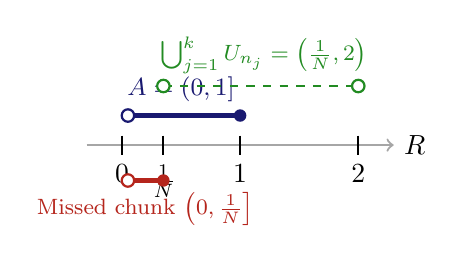
\begin{tikzpicture}[scale=1.5]
    % \begin{hidden}
    % - Canvas: scale 1.5, x in [-0.5, 2.4], y in [-0.4, 0.7]
    % - Elements: (1) real axis with ticks at 0, 1/N, 1, 2; (2) set A = (0, 1] with open circle at 0 and solid circle at 1;
    %   (3) finite subcover union (1/N, 2); (4) missed chunk (0, 1/N] in BrickRed; (5) labels
    % - Key coordinates: 0 at x = 0, 1/N at x = 0.35, 1 at x = 1.0, 2 at x = 2.0
    % - Collision check: all labels vertically separated, clear of horizontal axis lines
    % \end{hidden}
    \draw[thick, ->, gray!70] (-0.3, 0) -- (2.3, 0) node[right, text=black] {$\mathbb{R}$};

    % Axis ticks
    \draw[thick] (0, 0.08) -- (0, -0.08) node[below] {$0$};
    \draw[thick] (0.35, 0.08) -- (0.35, -0.08) node[below] {$\frac{1}{N}$};
    \draw[thick] (1.0, 0.08) -- (1.0, -0.08) node[below] {$1$};
    \draw[thick] (2.0, 0.08) -- (2.0, -0.08) node[below] {$2$};

    % Set A = (0, 1]
    \draw[ultra thick, MidnightBlue] (0.05, 0.25) -- (1.0, 0.25);
    \draw[thick, MidnightBlue, fill=white] (0.05, 0.25) circle (1.5pt);
    \fill[MidnightBlue] (1.0, 0.25) circle (1.5pt);
    \node[MidnightBlue, above, font=\small] at (0.5, 0.28) {$A = (0, 1]$};

    % Finite subcover union (1/N, 2)
    \draw[thick, ForestGreen, dashed] (0.35, 0.5) -- (2.0, 0.5);
    \draw[thick, ForestGreen, fill=white] (0.35, 0.5) circle (1.5pt);
    \draw[thick, ForestGreen, fill=white] (2.0, 0.5) circle (1.5pt);
    \node[ForestGreen, above, font=\footnotesize] at (1.2, 0.52) {$\bigcup_{j=1}^k U_{n_j} = \left(\frac{1}{N}, 2\right)$};

    % Missed chunk (0, 1/N]
    \draw[ultra thick, BrickRed] (0.05, -0.3) -- (0.35, -0.3);
    \draw[thick, BrickRed, fill=white] (0.05, -0.3) circle (1.5pt);
    \fill[BrickRed] (0.35, -0.3) circle (1.5pt);
    \node[BrickRed, below, font=\footnotesize] at (0.2, -0.32) {Missed chunk $\left(0, \frac{1}{N}\right]$};
\end{tikzpicture}
\end{center}

\begin{steps}[The Student Misconception on Trivial Covers]
The lecturer highlights a fundamental logical fallacy that frequently confuses students:
\begin{itemize}
    \item A student might observe that the single open interval $V = (-1, 2)$ covers $A = (0, 1]$, and argue that $\{V\}$ is a finite subcover.
    \item \textbf{Why this argument fails:} Compactness demands that \textbf{every} open cover must possess a finite subcover ($\forall \mathcal{U} \ \exists \mathcal{U}_{\text{fin}}$). Showing that \emph{one particular} cover can be made finite is mathematically vacuous (indeed, the entire space $X = \mathbb{R}$ covers any set in a single step). To disprove compactness, one only needs to exhibit a \textbf{single open cover} $\mathcal{U}$ that admits no finite subcover.
\end{itemize}
\end{steps}
\end{content}

\begin{speech}[01:11:26 - 01:12:47]
Speaking about open and closed, is there any question about compactness? We will see this more and more during the course, especially in the case of $\mathbb{R}^n$. So, you will get to know the notion of compactness much better and interiorize it, but now we needed some starting framework to start to use it.

And then the next thing in the list of topological notions that we want to study --- that you also learned a little bit in $\mathbb{R}$, but is much more interesting in a general metric space --- is connectedness. This starts to be new, and it's very nice. You will see that this is much more interesting. And new. Connectedness.
\end{speech}

\section{Connectedness}

\subsection{Preliminary: \texorpdfstring{\qt{Clopen}}{Clopen} Sets}

\begin{speech}[01:12:47 - 01:14:49]
Next topic: $(X, d)$ a metric space, and we will define connectedness, right? But before defining connectedness, I need a preliminary.

A preliminary observation \inlinemetanote{writes 'preliminary'} is that in any metric space, \inlinemetanote{writes 'In any metric space'} the whole set and the empty set \inlinemetanote{writes '$X, \emptyset$ are'} are always open and closed at the same time. \inlinemetanote{writes 'always open \& closed'}

Here, some authors call these sets \qt{clopen} because they are closed and open: clopen. \inlinemetanote{writes '[clopen]'}

In a given space, we will see that it's a rare property that in your space you have sets that are at the same time open and closed. And I'm saying this now because, first, some people asked during these days: is the whole space always open, or is the empty set closed or open? Okay.
\end{speech}

\begin{speech}[01:14:49 - 01:16:27]
So, let me say why this is true. First, what was the definition of an open set?

The definition of an open set is that for every point in my set, I can find a ball of positive radius, right? If my set is the whole space, the ball of radius $1$ for any point is in my space, tautologically. So, the whole set is always open.

Now, that the empty set is open is more arguable, if you want, right? Some books take it as an axiom that the empty set is open, but actually, if you use the logical consequence of the definition I gave, the empty set is open.

Because the definition I gave was: $U \subset X$ is open \inlinemetanote{writes '$U \subset X$ open if'} if for every $x$ in $U$, \inlinemetanote{writes '$\forall x \in U$'} something happens, right? And whenever you have an empty set, for every $x$ in $U$, anything you want happens, right? So, it is open, right?

Strictly speaking, it is covered by our definition. We don't need to impose any extra axiom. But if you want, just believe as an axiom that the empty set is open. \inlinemetanote{boxes the open definition on the board}
\end{speech}

\begin{content}[Preliminary: Clopen Sets]
In any metric space $(X, d)$, the empty set $\emptyset$ and the whole space $X$ are always both open and closed (often called \newterm{clopen} sets).
\begin{itemize}
    \item \textbf{The whole space $X$ is open:} For any point $x \in X$, any open ball of radius $r = 1$ is trivially contained within the space:
    \[
    \forall x \in X \ \exists r > 0 \colon \quad B_r(x) \subseteq X.
    \]
    Since $X$ is open, its complement $X^c = X \setminus X = \emptyset$ is closed.
    \item \textbf{The empty set $\emptyset$ is open:} The definition of openness holds vacuously for $\emptyset$:
    \[
    \forall x \in \emptyset \ \exists r > 0 \colon \quad B_r(x) \subseteq \emptyset.
    \]
    Since $\emptyset$ contains no elements, the universal condition over its elements is vacuously true. Since $\emptyset$ is open, its complement $\emptyset^c = X \setminus \emptyset = X$ is closed.
\end{itemize}

\begin{steps}[Vacuous Truth in Topology]
As the lecturer emphasizes, students often wonder whether $\emptyset$ being open is an arbitrary ad-hoc axiom. In formal first-order logic, the statement $\forall x \in \emptyset \colon P(x)$ is formally expressed as $\forall x \, (x \in \emptyset \implies P(x))$. Because the premise $x \in \emptyset$ is identically false for all $x$, the implication is true. Therefore, the openness of the empty set is a direct deductive consequence of the definition of an open set, requiring no extra axioms.
\end{steps}
\end{content}

\subsection{The Partition Problem on the Sphere \texorpdfstring{$S^2$}{S2}}

\begin{speech}[01:16:27 - 01:17:54]
And now, let me give a question for you. \inlinemetanote{writes 'Question:'}

Let's take $X$ to be the two-dimensional sphere, so call it $S^2$: \inlinemetanote{writes '$X = S^2 =$'} it's just the set of points $(x, y, z)$ in $\mathbb{R}^3$ such that $x^2 + y^2 + z^2 = 1$. \inlinemetanote{writes '$\{ (x, y, z) \in \mathbb{R}^3 : x^2 + y^2 + z^2 = 1 \}$'}

This is the unit sphere. And we take it with the restriction of the Euclidean distance: \inlinemetanote{writes '$d_{\text{Eucl}}|_X =: X$'} $d$ Euclidean restricted to my set $X$, right? We have already seen this example on one of the first days.

This is the drawing: a sphere. \inlinemetanote{draws a circle with equator line} I'm just putting this to make an interesting example that by now shouldn't be obvious, and in the next lecture the answer to this question I'm going to make will be obvious.
\end{speech}

\begin{speech}[01:17:54 - 01:19:58]
So, we have the sphere, and now I ask you: can you cover this sphere... in this set there are open and closed subsets, right? \inlinemetanote{writes 'open subsets'}

Here you have open subsets. And my question is: is it possible to write \inlinemetanote{writes 'Is it possible to write'} the sphere --- the whole space $X$, that is my sphere \inlinemetanote{writes '$X =$'} --- as a disjoint union, $U \cup V$, \inlinemetanote{writes '$U \cup V$'} meaning that $U \cap V$ is the empty set, \inlinemetanote{writes 'disjoint'} \inlinemetanote{writes '$(U \cap V = \emptyset)$'} and both are open and non-empty? \inlinemetanote{writes 'open, open, non-empty'}

Right?

Can you decompose your sphere as a union of two disjoint open sets? It doesn't look like it, but it's not clear a priori. So, you can intuitively say: no, this will be impossible. But to write a proof of this fact --- that for any pair of open sets I give, they will either have some intersection or maybe they don't cover, right? --- this looks complicated.

So, we will need more theory to find answers to this type of question. And you will see that this type of question we will use many times in Analysis 2 to prove that functions with zero derivative are constant in a connected set, and this kind of thing.
\end{speech}

\begin{content}[The Sphere Partition Question]
\begin{question}[Partitioning the 2-Sphere]\label[question]{q:sphere-partition}
Let $X = S^2 \subset \mathbb{R}^3$ be the two-dimensional unit sphere equipped with the subspace Euclidean metric:
\[
S^2 := \left\{ (x, y, z) \in \mathbb{R}^3 \;\middle|\; x^2 + y^2 + z^2 = 1 \right\}, \qquad d_{S^2} := d_{\text{Euclidean}}|_{S^2 \times S^2}.
\]
Is it possible to partition $S^2$ into a disjoint union of two non-empty, open subsets $U, V \subset S^2$? That is:
\begin{equation}\label{eq:sphere-decomposition}
S^2 = U \cup V \quad \text{with} \quad U \cap V = \emptyset, \quad U \neq \emptyset, \ V \neq \emptyset, \quad U, V \text{ open in } S^2.
\end{equation}
\end{question}

\begin{center}
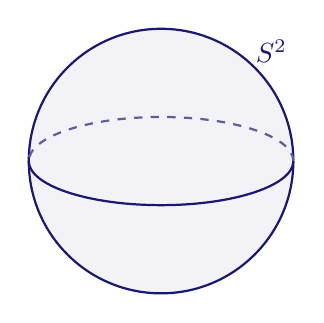
\begin{tikzpicture}[scale=1.4]
    % \begin{hidden}
    % - Canvas: scale 1.4, sphere radius 1.2 centered at (0,0)
    % - Elements: (1) light translucent fill; (2) outer circle outline; (3) back equator (dashed);
    %   (4) front equator (solid); (5) label S^2
    % - Coordinates: equator has horizontal radius 1.2, vertical radius 0.4
    % - Collisions: label placed at top-right outside the outline
    % \end{hidden}
    \fill[MidnightBlue!8, opacity=0.7] (0,0) circle (1.2cm);
    \draw[thick, MidnightBlue] (0,0) circle (1.2cm);
    \draw[dashed, MidnightBlue!70, thick] (1.2,0) arc (0:180:1.2cm and 0.4cm);
    \draw[thick, MidnightBlue] (-1.2,0) arc (180:360:1.2cm and 0.4cm);
    \node[MidnightBlue, font=\bfseries] at (1.0, 1.0) {$S^2$};
\end{tikzpicture}
\end{center}

\begin{steps}[Topological Intuition Behind the Question]
Intuitively, the sphere $S^2$ is an unbroken geometric surface consisting of a single continuous piece. Decomposing it into two disjoint open pieces without leaving any boundary seam between them seems impossible because open sets cannot contain their boundary points. This fundamental geometric property of being \qt{in one piece} is what the mathematical concept of \newterm{connectedness} rigorously captures.
\end{steps}
\end{content}

\begin{hidden}
% timestamp: 00:17:30
% topic: Partition problems on S^2 and intervals in R
% board_state: q:sphere-partition, eq:sphere-decomposition
% next_goal: Introduce the 1D interval partition analogue and define connectedness
% open_loops: is S^2 connected? (to be answered in future lectures)
\end{hidden}

\subsection{The Partition Problem for Intervals in \texorpdfstring{$\mathbb{R}$}{R}}

\begin{speech}[01:19:58 - 01:21:49]
Okay, so maybe now I can define...

I have put this question on the sphere to make it a bit more difficult to think about, right? And I wanted to give this example to say: something that now is difficult to think of, in a lecture, when you have more theory, you will see the answer clearly; you will have a one-line answer to this.

But you can pose the same question when $X$ is some interval in $\mathbb{R}$: \inlinemetanote{writes 'Same question when $X = (0, 1) \subset \mathbb{R}$'} when $X$ is, let's say, the interval $(0, 1)$ in $\mathbb{R}$.

Can you decompose the interval $(0, 1)$ in $\mathbb{R}$ as the disjoint union of two non-empty open sets, right?

If one of the sets is closed and the other open, yes, because you can say: okay, $(0, 1)$ I can put as the union of $(0, 1/2]$ --- close this one --- union $(1/2, 1)$, right? \inlinemetanote{writes '$(0, 1) = (0, 1/2] \cup (1/2, 1)$'} The $1/2$ you can put in this one. But this will not be open.

So, the question is: can we decompose a set into a disjoint union of open sets? And this question motivates the definition of connectedness.
\end{speech}

\begin{content}[The Partition Problem on Real Intervals]
\begin{question}[Partitioning $(0, 1)$ into Open Sets]\label[question]{q:interval-partition}
Can the open interval $(0, 1) \subset \mathbb{R}$ be decomposed into two disjoint, non-empty open subsets $U, V \subset (0, 1)$?
\end{question}

\textbf{Analysis of a Candidate Partition:}
If we drop the requirement that both sets must be open, a disjoint partition is elementary:
\[
(0, 1) = \left( 0, \frac{1}{2} \right] \cup \left( \frac{1}{2}, 1 \right).
\]
However, while $\left(\frac{1}{2}, 1\right)$ is open in $(0, 1)$, the subset $\left(0, \frac{1}{2}\right]$ is not open in $(0, 1)$ because any open ball in $\mathbb{R}$ centered at $x = \frac{1}{2}$ contains points strictly greater than $\frac{1}{2}$. Thus, this does not yield a partition into two open sets.
\end{content}

\begin{note}[Board Transition]
The lecturer takes a wet sponge and erases the bottom-right blackboard panel from 00:19:40 to 00:20:06 to prepare for writing the formal definitions of disconnected and connected sets.
\end{note}

\subsection{Formal Definition of Connectedness}

\begin{speech}[01:22:15 - 01:24:03]
...is called connected... \inlinemetanote{writes 'Def: Given $(X, d)$ metric space, $A \subset X$ (non-empty)'} Sorry, first I will define connected by saying what is disconnected, so what is the contrary. So, this definition will be by opposition to the concept of disconnected.

So, I will define first disconnected: \inlinemetanote{writes 'disconnected if'} a subset is disconnected if there exist $U$ and $V$ open, \inlinemetanote{writes '$\exists U, V$ open'} disjoint, \inlinemetanote{writes 'disjoint'} and non-empty, \inlinemetanote{writes 'and non-empty'} such that $A$ is contained in $U \cup V$, \inlinemetanote{writes 'such that $A \subset U \cup V$'} and both $A \cap U$ is non-empty \inlinemetanote{writes 'and $A \cap U \neq \emptyset$'} and $A \cap V$ is non-empty. \inlinemetanote{writes 'and $A \cap V \neq \emptyset$'}

This is the definition of a disconnected set, right?
\end{speech}

\begin{content}[Definition of Disconnected Subsets]
Let $(X, d)$ be a metric space.

\begin{definition}[Disconnected Set]\label[definition]{def:disconnected-set}
A non-empty subset $A \subseteq X$ is called \newterm{disconnected} if there exist open subsets $U, V \subseteq X$ such that:
\begin{enumerate}[label=\textbf{(\roman*)}]
    \item $U \cap V = \emptyset$ (i.e., $U$ and $V$ are disjoint),
    \item $A \subseteq U \cup V$ (i.e., $U$ and $V$ cover $A$),
    \item $A \cap U \neq \emptyset$ and $A \cap V \neq \emptyset$ (i.e., both open sets intersect $A$).
\end{enumerate}
The pair $(U, V)$ is called a \newterm{separation} (or disconnection) of $A$.
\end{definition}
\end{content}

\subsection{Examples of Disconnected Sets}

\begin{speech}[01:24:03 - 01:24:33]
And now let's go to the space you control very, very well, that is $\mathbb{R}$, and give me some example of a disconnected set.

What is the easiest example you can think of of a disconnected set?
\end{speech}

\begin{student}[Student Answer]
Open interval from $0$ to $1$ union open interval from $0$ to---from $2$ to $3$?
\end{student}

\begin{speech}[01:24:37 - 01:25:29]
Yes! So, this is an example. \inlinemetanote{writes 'In $\mathbb{R}$, set $A = (0, 1) \cup (2, 3)$'}

So, this is an open disconnected set: $(0, 1) \cup (2, 3)$. By construction, this set is the disjoint union of two open sets, right? Non-empty. Then, it is disconnected.

I can also say: if I take the set $\{0\}$ and $\{1\}$, \inlinemetanote{writes '$A = \{0, 1\}$'} two points, this is always a disconnected set, because I have the set $\{0\}$ and the set $\{1\}$, and I can take two open sets like this that disconnect the set, right? \inlinemetanote{draws intervals disconnecting $\{0\}$ and $\{1\}$}
\end{speech}

\begin{content}[Examples of Disconnected Sets in $\mathbb{R}$]
\begin{example}[Disconnected Subsets of $\mathbb{R}$]\label[example]{ex:disconnected-sets}
\begin{enumerate}[label=\textbf{(\arabic*)}]
    \item \textbf{Disjoint Open Intervals:}
    Let $A := (0, 1) \cup (2, 3) \subset \mathbb{R}$.
    Choosing $U := (0, 1)$ and $V := (2, 3)$, both $U$ and $V$ are open in $\mathbb{R}$, $U \cap V = \emptyset$, and:
    \[
    A \subseteq U \cup V, \qquad A \cap U = (0, 1) \neq \emptyset, \qquad A \cap V = (2, 3) \neq \emptyset.
    \]
    Thus, $A$ is disconnected.
    \item \textbf{A Discrete Two-Point Set:}
    Let $A := \{0, 1\} \subset \mathbb{R}$.
    Choosing open neighborhoods $U := \left(-\frac{1}{2}, \frac{1}{2}\right)$ and $V := \left(\frac{1}{2}, \frac{3}{2}\right)$, we have $U \cap V = \emptyset$, $0 \in U$, $1 \in V$, and $A \subset U \cup V$. Hence, $\{0, 1\}$ is disconnected.
\end{enumerate}
\end{example}

\begin{center}
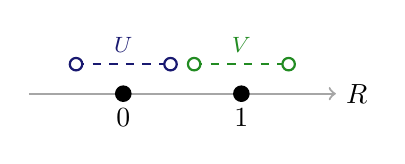
\begin{tikzpicture}[scale=1.5]
    % \begin{hidden}
    % - Canvas: scale 1.5, x in [-0.8, 1.8], y in [-0.1, 0.45]
    % - Elements: (1) real axis; (2) points 0 and 1; (3) dashed intervals U and V separating the points
    % - Coordinates: 0 at x = 0, 1 at x = 1. U = (-0.4, 0.4), V = (0.6, 1.4)
    % \end{hidden}
    \draw[thick, ->, gray!70] (-0.8, 0) -- (1.8, 0) node[right, text=black] {$\mathbb{R}$};

    % Points 0 and 1
    \fill[black] (0, 0) circle (2pt) node[below=2pt] {$0$};
    \fill[black] (1, 0) circle (2pt) node[below=2pt] {$1$};

    % Separating neighborhoods U and V
    \draw[thick, MidnightBlue, dashed] (-0.4, 0.25) -- (0.4, 0.25);
    \draw[thick, MidnightBlue, fill=white] (-0.4, 0.25) circle (1.5pt);
    \draw[thick, MidnightBlue, fill=white] (0.4, 0.25) circle (1.5pt);
    \node[MidnightBlue, above, font=\footnotesize] at (0, 0.27) {$U$};

    \draw[thick, ForestGreen, dashed] (0.6, 0.25) -- (1.4, 0.25);
    \draw[thick, ForestGreen, fill=white] (0.6, 0.25) circle (1.5pt);
    \draw[thick, ForestGreen, fill=white] (1.4, 0.25) circle (1.5pt);
    \node[ForestGreen, above, font=\footnotesize] at (1, 0.27) {$V$};
\end{tikzpicture}
\end{center}
\end{content}

\subsection{Definition of Connected Sets}

\begin{speech}[01:25:29 - 01:26:52]
And then I will define a connected set as any set that is not disconnected.

We say $A$ is connected if it is NOT disconnected. \inlinemetanote{writes 'We say $A$ is connected if it is NOT disconnected.'}

So, this means that whenever I have two open sets that cover it and are disjoint, one of them will be empty, right?

So, a set is connected if, whenever I can cover it by a union of open sets that are disjoint, necessarily one of them will have empty intersection with my set. And with this definition, we will prove next time several things. \inlinemetanote{students applaud and lecturer packs up his notes}
\end{speech}

\begin{content}[Definition of Connected Subsets]
\begin{definition}[Connected Set]\label[definition]{def:connected-set}
A non-empty subset $A \subseteq X$ is called \newterm{connected} if it is not disconnected.

Equivalently, $A$ is connected if whenever $U, V \subseteq X$ are open subsets satisfying $U \cap V = \emptyset$ and $A \subseteq U \cup V$, we must have:
\[
A \cap U = \emptyset \quad \text{or} \quad A \cap V = \emptyset.
\]
\end{definition}

\begin{steps}[Conceptual Summary of Connectedness]
Connectedness is formulated as the logical negation of disconnectedness:
\begin{itemize}
    \item A set is \textbf{disconnected} if it can be split into two non-overlapping open pieces.
    \item A set is \textbf{connected} if no such two-piece open separation exists. That is, whenever two disjoint open sets cover $A$, the set $A$ must be contained entirely within one of them.
\end{itemize}
\end{steps}
\end{content}

\begin{overview}[Summary of Key Concepts]
\begin{itemize}
    \item \textbf{Equivalence of Compactness Notions:} In any metric space $(X, d)$, a subset $K$ is sequentially compact if and only if it is topologically compact (open covers admit finite subcovers).
    \item \textbf{General Metric Consequences:} Compact sets are automatically closed and complete, their closed subsets remain compact, and their continuous images are compact.
    \item \textbf{Extreme Value Theorem:} Every real-valued continuous function $f \colon K \to \mathbb{R}$ on a compact metric space is bounded and attains its global maximum and minimum on $K$.
    \item \textbf{Heine--Borel Theorem in $\mathbb{R}^n$:} In Euclidean space, a subset is compact if and only if it is closed and bounded. Boundedness allows reduction to compact cubes $[-N, N]^n$, which are shown to be compact via coordinate-wise Bolzano--Weierstrass extractions.
    \item \textbf{Connectedness:} Subsets that cannot be partitioned into two disjoint, non-empty open sets are connected. The entire space $X$ and the empty set $\emptyset$ are always clopen in any metric space.
\end{itemize}
\end{overview}